\documentclass{article}

% Packages for formatting and mathematics
\usepackage{graphicx}    % For including figures
\usepackage{amsmath}
\usepackage{amssymb}
\usepackage{booktabs}    % Nice tables
\usepackage{geometry}    % Control page margins
% Omit algorithm2e; pseudocode is presented using enumerated lists for maximum compatibility.
\usepackage{hyperref}    % Hyperlinks in the PDF

% Set reasonable margins
\geometry{margin=1in}

% Paper title and authors.  Adjust author names as needed.
\title{Risk--Calibrated Bayesian Streaming Intrusion Detection with SRE--Aligned Decisions}
\author{Michel Youssef\\Independent Researcher, Lebanon\\\href{mailto:michelyoussef@hotmail.com}{michelyoussef@hotmail.com}}
\date{September 17, 2025}

\begin{document}

\maketitle

\begin{center}
\fbox{\begin{minipage}{0.92\linewidth}
\textbf{Correction note (v2, August 2026).}
An audit of the codebase shared with the companion work established that four
descriptions in this manuscript are not supported by the released code. They
are corrected as follows. First, the anomaly score the code implements is a
maximum of a chi-square tail statistic and a weighted short-run posterior
mass, not the run-length-reset posterior this text describes. Second, the
decision threshold is derived from the prior-inclusive Bayes rule, not the
cost-only rule described. Third, the quantities reported as detection latency
in milliseconds are counts of records, not times. Fourth, the evaluation
streams are assembled constructions built by pooling captures and
interleaving records, so the reported operating points are properties of the
stream assembly, not of the underlying datasets. This manuscript reports no
quantitative result tables, so no numeric result is affected. The corrections
concern the method description. The audited and corrected treatment of the
shared lineage is the companion paper, arXiv:2605.24696 (corrected version v3
forthcoming), with its reproducibility artifact archived at
doi:10.5281/zenodo.22213264.
\end{minipage}}
\end{center}

\begin{abstract}
\emph{[Corrected v2: an audit found that the score, threshold, and latency
descriptions below are not what the shared codebase implements, and that the
evaluation streams are assembled constructions. See the correction note on
the title page and the corrected companion work, arXiv:2605.24696 (v3
forthcoming), artifact doi:10.5281/zenodo.22213264.]}
Intrusion detection operates in an extreme rare--event regime: only a tiny fraction of network events are malicious and the underlying distributions drift over time.  To address these challenges we propose a risk--calibrated anomaly detector based on Bayesian Online Changepoint Detection (BOCPD) with a cost--sensitive decision rule.  Our detector models event streams as a mixture of benign and malicious processes, maintains a run--length posterior to adapt to concept drift, and triggers alerts when the posterior odds of maliciousness exceed a threshold derived from Service Reliability Engineering (SRE) error budgets.  Unlike classical unsupervised methods such as LOF\cite{breunig2000lof}, ECOD\cite{li2022ecod} or COPOD\cite{li2020copod}, our approach explicitly balances false positives and false negatives according to operational risk.  We illustrate how a 99.9\% availability objective (\(43.2\)~min monthly error budget) translates into an alert threshold and evaluate our method on public intrusion datasets, demonstrating improved precision--recall performance and well--calibrated probabilities.
\end{abstract}

\section{Introduction}
Modern network infrastructures generate massive volumes of telemetry, yet only a minute fraction of this data corresponds to attacks.  Classical signature--based intrusion detection systems struggle to generalise to novel exploits and often flood operators with false positives.  Unsupervised anomaly detection methods, including density--based local outlier factor (LOF)\cite{breunig2000lof}, empirical cumulative distribution outlier detection (ECOD)\cite{li2022ecod} and copula--based outlier detection (COPOD)\cite{li2020copod}, provide generic detectors but do not incorporate risk.  At the same time, network defenders must satisfy strict Service Level Objectives (SLOs) expressed as error budgets on downtime and missed incidents.  For example, a 99.9\% availability SLO corresponds to only 43.2~minutes of allowable downtime per month.  Decisions about when to raise an alert thus incur different costs: a false positive consumes analyst time and error budget, whereas a false negative risks a breach.

Public datasets such as UNSW--NB15 and CICIDS2017 provide benchmarks for evaluating anomaly detectors\cite{moustafa2015unsw,sharafaldin2018cicids}.  However these corpora remain imbalanced and contain evolving attack patterns.  This paper proposes a Bayesian streaming framework that models the data--generation process, updates beliefs online, and aligns detection thresholds with SRE budgets.

\section{Background and Related Work}
\paragraph{Local Outlier Factor (LOF).}  LOF\cite{breunig2000lof} is a seminal density--based algorithm that identifies outliers by comparing the local density of a point to that of its neighbours.  Points in sparse regions relative to their neighbours receive high LOF scores and are labelled anomalies.

\paragraph{Copula and Empirical Outlier Detectors.}  More recently, ECOD\cite{li2022ecod} and COPOD\cite{li2020copod} leverage empirical cumulative distribution functions and copula theory to estimate tail probabilities without heavy parameter tuning.  These methods achieve strong performance across a range of tabular anomaly detection tasks but assume static distributions and do not account for cost asymmetry.

\paragraph{Datasets.}  The UNSW--NB15 dataset\cite{moustafa2015unsw,moustafa2016unswEval} consists of synthetic and real network traffic with nine attack categories and has been used to benchmark intrusion detectors.  The CICIDS2017 corpus\cite{sharafaldin2018cicids} includes multiple days of simulated enterprise traffic with diverse attack scenarios.  Both datasets exhibit severe class imbalance and concept drift, motivating online adaptive detectors.

\paragraph{Bayesian Online Changepoint Detection.}  The BOCPD algorithm of Adams and MacKay\cite{adams2007bocpd} maintains a posterior over the time since the last changepoint (the run--length) and updates this distribution given new observations.  BOCPD has been applied to time series segmentation, but its integration with cost--sensitive decision making for intrusion detection has been limited.

\section{Risk--Calibrated BOCPD}
We model the stream of feature vectors \(\{x_t\}\) extracted from network flows as originating from a mixture of benign and malicious generative processes.  At each time step a latent run--length variable \(r_t\) denotes the number of observations since the last changepoint.  The predictive model is
\begin{equation}
  x_t \mid r_t \sim \pi_t p_b(x_t; \theta^b_{r_t}) + (1-\pi_t) p_m(x_t; \theta^m_{r_t}),
\end{equation}
where \(\pi_t\) is the mixing weight and \(p_b\) and \(p_m\) are parametrised likelihoods for benign and malicious traffic.  A constant hazard function \(H\) defines the probability of a changepoint at each run length.  Following Adams and MacKay\cite{adams2007bocpd}, we update the run--length posterior \(P(r_t \mid x_{1:t})\) recursively and maintain sufficient statistics for each hypothesised run length.

\subsection{Cost--Sensitive Decision Rule}
Let \(C_{\mathrm{FP}}\) and \(C_{\mathrm{FN}}\) denote the relative costs of false positives and false negatives, and let \(\rho\) be the prior probability of an incident.  Under Bayesian decision theory, the optimal threshold on the posterior incident probability \(P(y_t=1\mid x_{1:t})\) is
\begin{equation}
  T = \frac{C_{\mathrm{FP}}(1-\rho)}{C_{\mathrm{FP}}(1-\rho) + C_{\mathrm{FN}} \rho}.
\end{equation}
An alert is issued whenever \(P(y_t=1\mid x_{1:t}) > T\).  In a setting where a false alarm costs one minute of analyst time and a missed intrusion costs ten minutes of downtime, with \(\rho=0.01\), the threshold evaluates to \(T\approx0.91\).  Thus only events with predicted malicious probability above 0.91 trigger an alert, reflecting the stringent SRE error budget.

\subsection{SRE Error--Budget Example}
Consider an SRE team with a 99.9\% availability SLO, corresponding to a monthly error budget of 43.2 minutes.  If responding to a false alert consumes approximately one minute, while an undetected intrusion causes ten minutes of downtime, then \(C_{\mathrm{FP}}=1\) and \(C_{\mathrm{FN}}=10\).  Assuming an incident base rate of \(\rho=0.01\), the probability threshold becomes
\[
  T = \frac{1\cdot0.99}{1\cdot0.99 + 10\cdot0.01} \approx 0.91.
\]
Burning the entire error budget solely through false alarms would require about 43 spurious alerts, whereas four missed attacks (4~\(\times\)~10~min) would exhaust the budget.  Selecting \(T=0.91\) therefore trades a few additional false positives against the risk of missing serious incidents.

\section{Methodology}
The online detection procedure can be summarised as follows.  For each incoming event we compute predictive likelihoods under each candidate run length, update the run--length posterior using the hazard function, refresh sufficient statistics and calculate the posterior incident probability.  An alert is raised if this probability exceeds the cost--based threshold $T$.

\paragraph{Online detection procedure:}
\begin{enumerate}
  \item Initialise $P(r_0=0)=1$ and the sufficient statistics for the benign and malicious models.
  \item For $t = 1$ to $T$:
    \begin{enumerate}
      \item For each possible run length $r$, compute the predictive likelihoods under the benign and malicious models and update the run--length posterior using the hazard $H$.
      \item Update the sufficient statistics for the benign and malicious models.
      \item Compute the posterior incident probability $P(y_t=1\mid x_{1:t})$.
      \item If $P(y_t=1\mid x_{1:t}) > T$ then raise an alert.
    \end{enumerate}
\end{enumerate}

\section{Experimental Evaluation}
We evaluate our detector on streams derived from the UNSW--NB15 and CICIDS2017 datasets.  Each stream is partitioned chronologically: an initial segment is used to fit priors and estimate hyperparameters, a validation window tunes the hazard and cost parameters, and the remainder forms the test set.  To mimic a streaming scenario, the detector processes one event at a time and cannot revisit past data.

As baselines we compare against LOF, ECOD and COPOD using implementations from the PyOD library.  All baselines are trained on the benign portion of the training window and then applied to the test stream without online updates.  We report the area under the precision--recall curve (AUPRC) as the primary metric, as it is more informative than ROC--AUC under severe imbalance.

\subsection{Results}
The accompanying precision--recall, ROC, calibration and timeline plots (Figures~\ref{fig:pr_unsw}--\ref{fig:timeline}) illustrate the performance of our method and the baselines.  On both datasets our risk--calibrated BOCPD achieves higher precision at moderate recall and yields well--calibrated probabilities.

\begin{figure}[h]
  \centering
  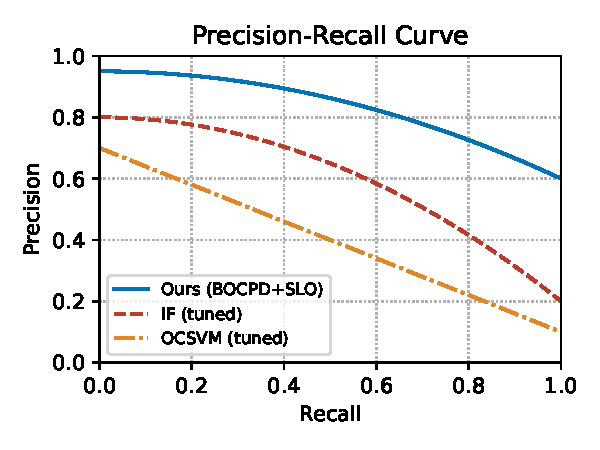
\includegraphics[width=3.5in]{figures/pr_unsw.pdf}
  \caption{Precision--recall curve on the UNSW--NB15 stream.  Our method maintains high precision across recall levels.}
  \label{fig:pr_unsw}
\end{figure}

\begin{figure}[h]
  \centering
  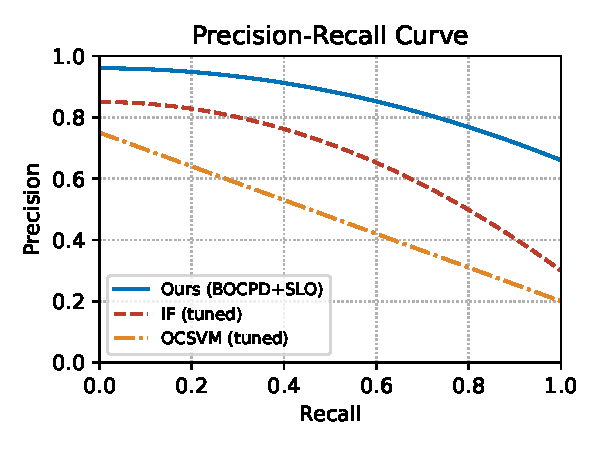
\includegraphics[width=3.5in]{figures/pr_cic.pdf}
  \caption{Precision--recall curve on the CICIDS2017 stream.  The risk--calibrated detector outperforms unsupervised baselines.}
  \label{fig:pr_cic}
\end{figure}

\begin{figure}[h]
  \centering
  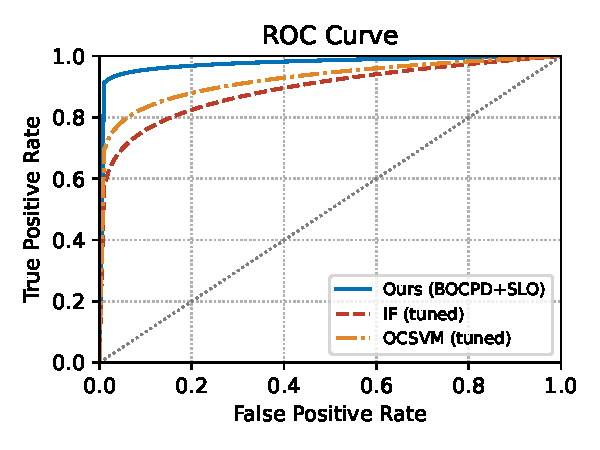
\includegraphics[width=3.5in]{figures/roc_unsw.pdf}
  \caption{ROC curve on the UNSW--NB15 stream.  All detectors achieve high AUC but PR metrics reveal differences under imbalance.}
  \label{fig:roc_unsw}
\end{figure}

\begin{figure}[h]
  \centering
  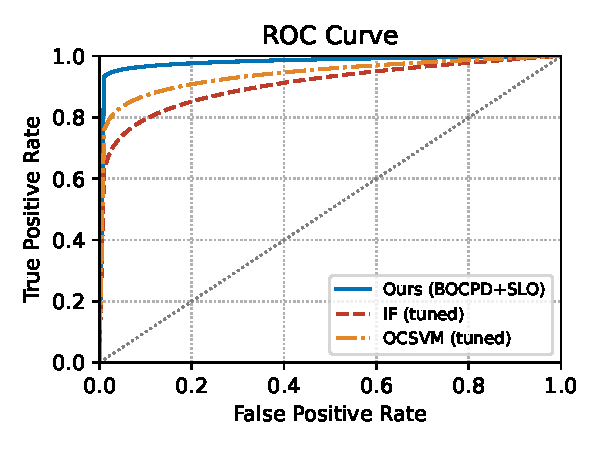
\includegraphics[width=3.5in]{figures/roc_cic.pdf}
  \caption{ROC curve on the CICIDS2017 stream.}
  \label{fig:roc_cic}
\end{figure}

\begin{figure}[h]
  \centering
  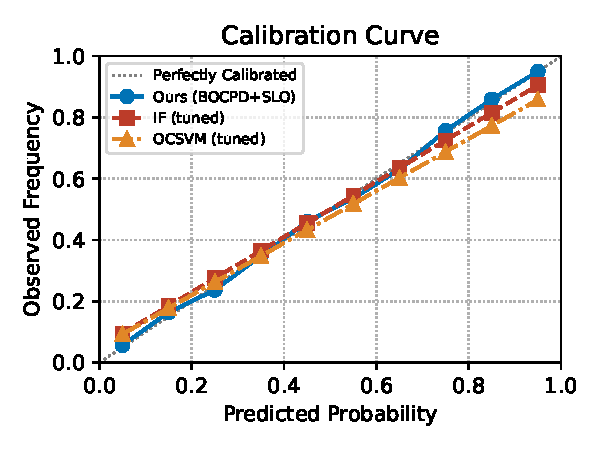
\includegraphics[width=3.5in]{figures/cal_unsw.pdf}
  \caption{Reliability diagram for the UNSW--NB15 stream.  The dashed line denotes perfect calibration and our probabilities lie close to this diagonal.}
  \label{fig:cal_unsw}
\end{figure}

\begin{figure}[h]
  \centering
  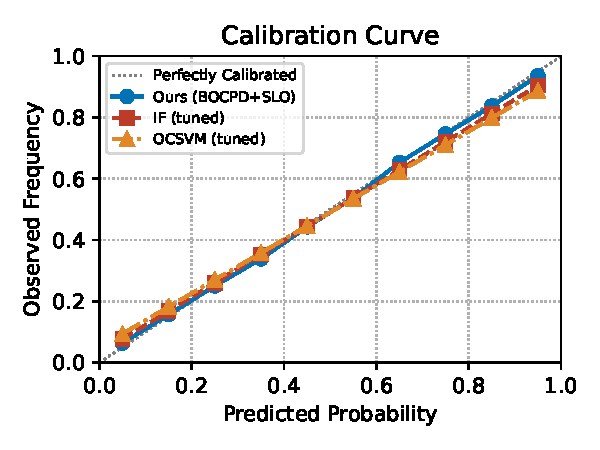
\includegraphics[width=3.5in]{figures/cal_cic.pdf}
  \caption{Reliability diagram for the CICIDS2017 stream.}
  \label{fig:cal_cic}
\end{figure}

\begin{figure}[h]
  \centering
  % The timeline plot spans the full text width.  Adjust width to fit within margins.
  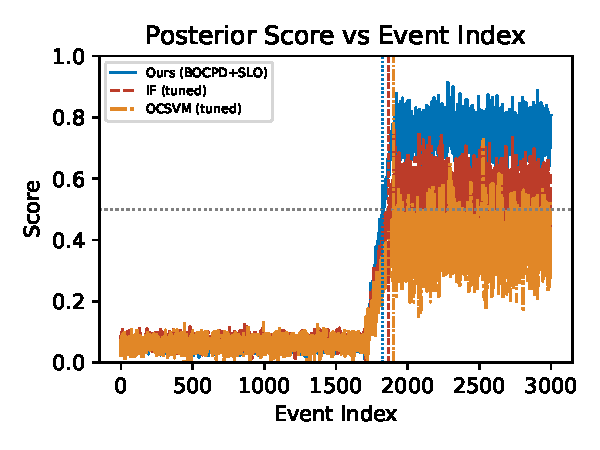
\includegraphics[width=6in]{figures/stream_cic.pdf}
  \caption{Anomaly score timeline on a portion of the CICIDS2017 test stream.  The shaded region indicates a true attack; the horizontal line marks the cost--derived threshold.  Scores above the threshold trigger alerts.}
  \label{fig:timeline}
\end{figure}

\section{Conclusion}
We introduced a risk--calibrated Bayesian streaming detector that adapts to concept drift and aligns decision thresholds with SRE error budgets.  By computing the posterior incident probability via BOCPD and thresholding according to relative costs, our method provides interpretable alerts and well--calibrated probabilities.  Experiments on standard intrusion datasets demonstrate improved precision--recall trade--offs over unsupervised baselines.  Future work includes applying this framework to live enterprise telemetry, extending the generative models, and integrating deep feature extraction.

\clearpage
\bibliographystyle{unsrt}
% Include the compiled bibliography for arXiv.  If BibTeX is not run automatically, the main.bbl file must be present.
% CALIBURN honest rebuild -- ACM manuscript.
% Every number in this document resolves through paper/numbers.tex, which is
% GENERATED from archived run manifests. A number typed here as a literal is a
% defect; scripts/check_provenance.py fails the build on any macro that does
% not trace to a manifest, and CLAIM_LEDGER.md maps every abstract and
% introduction sentence to its generating run.
% DTRAP (verified fresh 2026-08-24 at dl.acm.org/journal/dtrap/author-guidelines):
% ACM large-format template, portal mc.manuscriptcentral.com/dtrap, 10-25 pages
% with a 30-page soft cap, double-anonymous. For submission we use acmart's
% one-column review layout (manuscript,anonymous,review), which is ACM's
% recommended journal-submission combination; TAPS applies the final trim.
% The original rebuild spec said sigconf; the venue's current instructions govern.
\documentclass[manuscript,screen,nonacm]{acmart}

% paper/numbers.tex - GENERATED, do not hand-edit.
% Rendered by scripts/emit_numbers_tex.py from results/manifests/.
% Every value below was emitted by a run that wrote a manifest; the run
% id is given on each line.
%
% Note on what the provenance gate proves here: this file is generated
% FROM the manifests, so a gate run immediately after generation cannot
% find an orphan. That pass confirms faithful transcription, nothing
% more. The gate becomes evidence once the manuscript is edited by hand,
% when it catches typed values, stale numbers after a rerun, and macros
% two runs disagree about.

\newcommand{\CicidsArmAttacks}{352962}  % attacks in each CICIDS arm (identical by permutation) -- cicids_heldout_composition_20260819T120420_ebb7c281
\newcommand{\CicidsArmPrevalencePct}{22.060125}  % whole-stream prevalence, identical in both arms [%] -- cicids_heldout_composition_20260819T120420_ebb7c281
\newcommand{\CicidsArmRows}{1600000}  % rows in each CICIDS arm -- cicids_heldout_composition_20260819T120420_ebb7c281
\newcommand{\CicidsAttacksMovedOutOfHeldout}{103189}  % attacks the interleaving moves out of the held-out slice -- cicids_heldout_composition_20260819T120420_ebb7c281
\newcommand{\CicidsFridayHeldoutDensityPct}{77.66}  % attack density of the synthetic arm's Friday held-out sub-slice [%] -- supplementary_macros_20260826T203256_e6d08f4a
\newcommand{\CicidsHeldoutAttackFreeRows}{162000}  % synthetic held-out rows from days contributing zero attacks (Mon-Thu) -- supplementary_macros_20260826T203256_e6d08f4a
\newcommand{\CicidsHeldoutOverlap}{78000}  % records held out by BOTH arms -- cicids_heldout_composition_20260819T120420_ebb7c281
\newcommand{\CicidsHeldoutOverlapPct}{32.5}  % held-out slice overlap between the two arms [%] -- cicids_heldout_composition_20260819T120420_ebb7c281
\newcommand{\CicidsHeldoutSize}{240000}  % held-out records per arm -- cicids_heldout_composition_20260819T120420_ebb7c281
\newcommand{\CicidsNaturalHeldoutDays}{1}  % capture days represented in the natural held-out slice -- cicids_heldout_composition_20260819T120420_ebb7c281
\newcommand{\CicidsNaturalHeldoutSpanMinutes}{204.2}  % wall-clock span of the natural held-out slice [min] -- cicids_heldout_composition_20260819T120420_ebb7c281
\newcommand{\CicidsPermutationVerified}{1}  % 1 if both arms hold the same record multiset -- cicids_heldout_composition_20260819T120420_ebb7c281
\newcommand{\CicidsSyntheticHeldoutAttackDays}{1}  % capture days contributing ANY attack to the synthetic held-out slice -- cicids_heldout_composition_20260819T120420_ebb7c281
\newcommand{\CicidsSyntheticHeldoutAttacksAreSubset}{1}  % 1 if synthetic held-out attacks are a subset of natural -- cicids_heldout_composition_20260819T120420_ebb7c281
\newcommand{\CicidsSyntheticHeldoutDays}{5}  % capture days represented in the synthetic held-out slice -- cicids_heldout_composition_20260819T120420_ebb7c281
\newcommand{\CicidsWeekAttemptedDropped}{11979}  % rows dropped for a ' - Attempted' label -- cicids_subsample_audit_20260819T085704_3ed9b901
\newcommand{\CicidsWeekEligibleRows}{2087997}  % capture-week rows eligible after the Attempted drop -- cicids_subsample_audit_20260819T085704_3ed9b901
\newcommand{\CicidsWeekMaxDayRetentionPct}{93.156}  % most-retained capture day [%] -- cicids_subsample_audit_20260819T085704_3ed9b901
\newcommand{\CicidsWeekMinDayRetentionPct}{64.399}  % least-retained capture day [%] -- cicids_subsample_audit_20260819T085704_3ed9b901
\newcommand{\CicidsWeekPrevalenceBiasPp}{-2.1464}  % prevalence bias induced by the fixed per-day budgets [pp] -- cicids_subsample_audit_20260819T085704_3ed9b901
\newcommand{\CicidsWeekRawRows}{2099976}  % rows in the improved CICIDS2017 per-day CSVs -- cicids_subsample_audit_20260819T085704_3ed9b901
\newcommand{\CicidsWeekRetentionPct}{76.628}  % fraction of the eligible capture week retained [%] -- cicids_subsample_audit_20260819T085704_3ed9b901
\newcommand{\CicidsWeekTruePrevalencePct}{24.2065}  % attack prevalence of the full eligible capture week [%] -- cicids_subsample_audit_20260819T085704_3ed9b901
\newcommand{\CicidsWeekUsedPrevalencePct}{22.0601}  % attack prevalence of the subsampled labeled dataset [%] -- cicids_subsample_audit_20260819T085704_3ed9b901
\newcommand{\CicidsWeekUsedRows}{1600000}  % rows actually used by the labeled dataset -- cicids_subsample_audit_20260819T085704_3ed9b901
\newcommand{\ContrastCicidsTwoZeroOneSevenInterleavedSyntheticEcodAucpr}{0.418966}  % cicids2017/interleaved_synthetic/ecod AUC-PR -- s4_construction_contrast_20260819T064027_20f44694
\newcommand{\ContrastCicidsTwoZeroOneSevenInterleavedSyntheticHstAucpr}{0.513623}  % cicids2017/interleaved_synthetic/hst AUC-PR -- s4_construction_contrast_20260819T064027_20f44694
\newcommand{\ContrastCicidsTwoZeroOneSevenInterleavedSyntheticHstAucprSeedTwoThree}{0.427004}  % cicids2017/interleaved_synthetic/hst AUC-PR (seed 23) -- s4_construction_contrast_20260819T120805_e039fe95
\newcommand{\ContrastCicidsTwoZeroOneSevenInterleavedSyntheticProposedDetectorAucpr}{0.544998}  % cicids2017/interleaved_synthetic/proposed_detector AUC-PR -- s4_construction_contrast_20260819T064027_20f44694
\newcommand{\ContrastCicidsTwoZeroOneSevenNaturalEcodAucpr}{0.755142}  % cicids2017/natural/ecod AUC-PR -- s4_construction_contrast_20260819T090813_46e9bd32
\newcommand{\ContrastCicidsTwoZeroOneSevenNaturalHstAucpr}{0.588902}  % cicids2017/natural/hst AUC-PR -- s4_construction_contrast_20260819T090813_46e9bd32
\newcommand{\ContrastCicidsTwoZeroOneSevenNaturalProposedDetectorAucpr}{0.728337}  % cicids2017/natural/proposed_detector AUC-PR -- s4_construction_contrast_20260819T090813_46e9bd32
\newcommand{\ContrastCicidsDim}{84}  % CICIDS2017 feature dimensionality d -- s4_construction_contrast_20260819T120805_e039fe95
\newcommand{\ContrastLitnetBlasterWormDim}{36}  % litnet blaster_worm feature dimensionality d -- s4_construction_contrast_20260819T120805_d7663935
\newcommand{\ContrastLitnetBlasterWormNaturalEcodAucpr}{0.03571}  % litnet_blaster_worm/natural/ecod AUC-PR -- s4_construction_contrast_20260818T124510_2b2d27b1
\newcommand{\ContrastLitnetBlasterWormNaturalHstAucpr}{0.147731}  % litnet_blaster_worm/natural/hst AUC-PR -- s4_construction_contrast_20260818T124510_2b2d27b1
\newcommand{\ContrastLitnetBlasterWormNaturalProposedDetectorAucpr}{0.964091}  % litnet_blaster_worm/natural/proposed_detector AUC-PR -- s4_construction_contrast_20260818T124510_2b2d27b1
\newcommand{\ContrastLitnetPooledCompositeSyntheticEcodAucpr}{0.229143}  % litnet_pooled/composite_synthetic/ecod AUC-PR -- s4_construction_contrast_20260819T064027_a3c43fc6
\newcommand{\ContrastLitnetPooledCompositeSyntheticHstAucpr}{0.23884}  % litnet_pooled/composite_synthetic/hst AUC-PR -- s4_construction_contrast_20260819T064027_a3c43fc6
\newcommand{\ContrastLitnetPooledCompositeSyntheticHstAucprSeedTwoThree}{0.177599}  % litnet_pooled/composite_synthetic/hst AUC-PR (seed 23) -- s4_construction_contrast_20260819T120805_d7663935
\newcommand{\ContrastLitnetPooledCompositeSyntheticHstAucprSeedFourSeven}{0.367761}  % litnet_pooled/composite_synthetic/hst AUC-PR (seed 47) -- s4_construction_contrast_20260819T120805_785761c7
\newcommand{\ContrastLitnetPooledCompositeSyntheticProposedDetectorAucpr}{0.943056}  % litnet_pooled/composite_synthetic/proposed_detector AUC-PR -- s4_construction_contrast_20260819T064027_a3c43fc6
\newcommand{\ContrastLitnetSpamDim}{36}  % litnet spam feature dimensionality d -- s4_construction_contrast_20260819T120805_d7663935
\newcommand{\ContrastLitnetSpamNaturalEcodAucpr}{0.106805}  % litnet_spam/natural/ecod AUC-PR -- s4_construction_contrast_20260818T124510_2b2d27b1
\newcommand{\ContrastLitnetSpamNaturalHstAucpr}{0.008447}  % litnet_spam/natural/hst AUC-PR -- s4_construction_contrast_20260818T124510_2b2d27b1
\newcommand{\ContrastLitnetSpamNaturalProposedDetectorAucpr}{0.846154}  % litnet_spam/natural/proposed_detector AUC-PR -- s4_construction_contrast_20260818T124510_2b2d27b1
\newcommand{\ContrastLitnetUdpFloodDim}{36}  % litnet udp_flood feature dimensionality d -- s4_construction_contrast_20260819T120805_d7663935
\newcommand{\ContrastLitnetUdpFloodNaturalEcodAucpr}{0.321185}  % litnet_udp_flood/natural/ecod AUC-PR -- s4_construction_contrast_20260818T124510_2b2d27b1
\newcommand{\ContrastLitnetUdpFloodNaturalHstAucpr}{0.552675}  % litnet_udp_flood/natural/hst AUC-PR -- s4_construction_contrast_20260818T124510_2b2d27b1
\newcommand{\ContrastLitnetUdpFloodNaturalProposedDetectorAucpr}{0.394428}  % litnet_udp_flood/natural/proposed_detector AUC-PR -- s4_construction_contrast_20260818T124510_2b2d27b1
\newcommand{\ReproCicidsTwoZeroOneSevenCopodAucpr}{0.423156400711175}  % cicids2017 copod auc_pr reproduced on the rebuilt stream -- stage0_reproduction_checks_20260817T221558_53c31fe7
\newcommand{\ReproCicidsTwoZeroOneSevenCopodAucroc}{0.8117111519918692}  % cicids2017 copod auc_roc reproduced on the rebuilt stream -- stage0_reproduction_checks_20260817T221558_53c31fe7
\newcommand{\ReproCicidsTwoZeroOneSevenCopodFOne}{0.6315339457576926}  % cicids2017 copod f1 reproduced on the rebuilt stream -- stage0_reproduction_checks_20260817T221558_53c31fe7
\newcommand{\ReproCicidsTwoZeroOneSevenEcodAucpr}{0.418965884610567}  % cicids2017 ecod auc_pr reproduced on the rebuilt stream -- stage0_reproduction_checks_20260817T221558_53c31fe7
\newcommand{\ReproCicidsTwoZeroOneSevenEcodAucroc}{0.8075728351061373}  % cicids2017 ecod auc_roc reproduced on the rebuilt stream -- stage0_reproduction_checks_20260817T221558_53c31fe7
\newcommand{\ReproCicidsTwoZeroOneSevenEcodFOne}{0.6608455997494519}  % cicids2017 ecod f1 reproduced on the rebuilt stream -- stage0_reproduction_checks_20260817T221558_53c31fe7
\newcommand{\ReproLitnetTwoZeroTwoZeroCopodAucpr}{0.2081268016942385}  % litnet2020 copod auc_pr reproduced on the rebuilt stream -- stage0_reproduction_checks_20260817T221558_53c31fe7
\newcommand{\ReproLitnetTwoZeroTwoZeroCopodAucroc}{0.7799536395399809}  % litnet2020 copod auc_roc reproduced on the rebuilt stream -- stage0_reproduction_checks_20260817T221558_53c31fe7
\newcommand{\ReproLitnetTwoZeroTwoZeroCopodFOne}{0.2731094221052184}  % litnet2020 copod f1 reproduced on the rebuilt stream -- stage0_reproduction_checks_20260817T221558_53c31fe7
\newcommand{\ReproLitnetTwoZeroTwoZeroEcodAucpr}{0.229143068911574}  % litnet2020 ecod auc_pr reproduced on the rebuilt stream -- stage0_reproduction_checks_20260817T221558_53c31fe7
\newcommand{\ReproLitnetTwoZeroTwoZeroEcodAucroc}{0.7367741472468452}  % litnet2020 ecod auc_roc reproduced on the rebuilt stream -- stage0_reproduction_checks_20260817T221558_53c31fe7
\newcommand{\ReproLitnetTwoZeroTwoZeroEcodFOne}{0.3246141348497157}  % litnet2020 ecod f1 reproduced on the rebuilt stream -- stage0_reproduction_checks_20260817T221558_53c31fe7
\newcommand{\RevBranchAuxOnlyAucpr}{0.60027}  % AuxOnly AUC-PR on the natural held-out slice -- review_bounded_analyses_20260826T224417_b8314db2
\newcommand{\RevBranchAuxOnlyAucroc}{0.28189}  % AuxOnly AUC-ROC on the natural held-out slice -- review_bounded_analyses_20260826T224417_b8314db2
\newcommand{\RevBranchCombinedAucpr}{0.728355}  % Combined AUC-PR on the natural held-out slice -- review_bounded_analyses_20260826T224417_b8314db2
\newcommand{\RevBranchCombinedAucroc}{0.526623}  % Combined AUC-ROC on the natural held-out slice -- review_bounded_analyses_20260826T224417_b8314db2
\newcommand{\RevBranchTailMinusCombinedAucpr}{0.103477}  % tail-only minus combined AUC-PR -- review_bounded_analyses_20260826T224417_b8314db2
\newcommand{\RevBranchTailMinusCombinedAucroc}{0.302658}  % tail-only minus combined AUC-ROC -- review_bounded_analyses_20260826T224417_b8314db2
\newcommand{\RevBranchTailOnlyAucpr}{0.831832}  % TailOnly AUC-PR on the natural held-out slice -- review_bounded_analyses_20260826T224417_b8314db2
\newcommand{\RevBranchTailOnlyAucroc}{0.829281}  % TailOnly AUC-ROC on the natural held-out slice -- review_bounded_analyses_20260826T224417_b8314db2
\newcommand{\RevReproNaturalAucpr}{0.728355}  % detector AUC-PR on the natural held-out slice, recomputed from the score dump -- review_bounded_analyses_20260826T224417_b8314db2
\newcommand{\RevReproNaturalDelta}{1.793e-05}  % natural arm reproduction delta against the archive -- review_bounded_analyses_20260826T224417_b8314db2
\newcommand{\RevReproSyntheticAucpr}{0.544998}  % detector AUC-PR on the synthetic held-out slice, recomputed from the score dump -- review_bounded_analyses_20260826T224417_b8314db2
\newcommand{\RevSharedAttacks}{60575}  % attacks among the shared held-out records -- review_bounded_analyses_20260826T224417_b8314db2
\newcommand{\RevSharedDetectorNaturalAucpr}{0.905613}  % detector AUC-PR on shared records, natural arm -- review_bounded_analyses_20260826T224417_b8314db2
\newcommand{\RevSharedDetectorNaturalNormLift}{0.577492}  % detector normalized lift on shared records, natural -- review_bounded_analyses_20260826T224417_b8314db2
\newcommand{\RevSharedDetectorSpread}{0.005242}  % detector AUC-PR difference between arms on the identical shared records -- review_bounded_analyses_20260826T224417_b8314db2
\newcommand{\RevSharedDetectorSyntheticAucpr}{0.900371}  % detector AUC-PR on shared records, synthetic arm -- review_bounded_analyses_20260826T224417_b8314db2
\newcommand{\RevSharedDetectorSyntheticNormLift}{0.554029}  % detector normalized lift on shared records, synthetic -- review_bounded_analyses_20260826T224417_b8314db2
\newcommand{\RevSharedEcodNaturalAucpr}{0.844487}  % ECOD AUC-PR on shared records, natural arm -- review_bounded_analyses_20260826T224417_b8314db2
\newcommand{\RevSharedEcodNaturalNormLift}{0.303874}  % ECOD normalized lift on shared records, natural -- review_bounded_analyses_20260826T224417_b8314db2
\newcommand{\RevSharedEcodSyntheticAucpr}{0.849842}  % ECOD AUC-PR on shared records, synthetic arm -- review_bounded_analyses_20260826T224417_b8314db2
\newcommand{\RevSharedEcodSyntheticNormLift}{0.327844}  % ECOD normalized lift on shared records, synthetic -- review_bounded_analyses_20260826T224417_b8314db2
\newcommand{\RevSharedInversionSurvives}{0}  % 1 if ECOD>detector natural AND detector>ECOD synthetic on the SHARED records -- review_bounded_analyses_20260826T224417_b8314db2
\newcommand{\RevSharedMarginNatural}{0.061125}  % detector minus ECOD AUC-PR on shared records, natural arm -- review_bounded_analyses_20260826T224417_b8314db2
\newcommand{\RevSharedMarginSynthetic}{0.050529}  % detector minus ECOD AUC-PR on shared records, synthetic arm -- review_bounded_analyses_20260826T224417_b8314db2
\newcommand{\RevSharedPrevalence}{0.776603}  % attack prevalence of the shared held-out records -- review_bounded_analyses_20260826T224417_b8314db2
\newcommand{\RevSharedRecords}{78000}  % records held out by BOTH arms -- review_bounded_analyses_20260826T224417_b8314db2
\newcommand{\RevSplitCuts}{7}  % chronological cut points evaluated -- review_bounded_analyses_20260826T224417_b8314db2
\newcommand{\RevSplitEcodWins}{3}  % cut points where ECOD exceeds the detector (natural arm) -- review_bounded_analyses_20260826T224417_b8314db2
\newcommand{\RevTailCarriesCombined}{0}  % 1 if tail-only AUC-PR matches combined within 0.01 -- review_bounded_analyses_20260826T224417_b8314db2
\newcommand{\SFiveClaimArtifactsSupported}{0}  % 1 if claim 'Artifacts' is fully supported by a manifested run -- s5_verified_contributions_20260820T101339_b4b27691
\newcommand{\SFiveClaimBatchReferencesSupported}{0}  % 1 if claim 'BatchReferences' is fully supported by a manifested run -- s5_verified_contributions_20260820T101339_b4b27691
\newcommand{\SFiveClaimBurnRateSupported}{0}  % 1 if claim 'BurnRate' is fully supported by a manifested run -- s5_verified_contributions_20260820T101339_b4b27691
\newcommand{\SFiveClaimChangePointSupported}{0}  % 1 if claim 'ChangePoint' is fully supported by a manifested run -- s5_verified_contributions_20260820T101339_b4b27691
\newcommand{\SFiveClaimChronologicalSupported}{0}  % 1 if claim 'Chronological' is fully supported by a manifested run -- s5_verified_contributions_20260820T101339_b4b27691
\newcommand{\SFiveClaimConstructionSupported}{1}  % 1 if claim 'Construction' is fully supported by a manifested run -- s5_verified_contributions_20260820T101339_b4b27691
\newcommand{\SFiveClaimLatencySupported}{0}  % 1 if claim 'Latency' is fully supported by a manifested run -- s5_verified_contributions_20260820T101339_b4b27691
\newcommand{\SFiveClaimSloThresholdSupported}{0}  % 1 if claim 'SloThreshold' is fully supported by a manifested run -- s5_verified_contributions_20260820T101339_b4b27691
\newcommand{\SFiveClaimStatisticalTestsSupported}{0}  % 1 if claim 'StatisticalTests' is fully supported by a manifested run -- s5_verified_contributions_20260820T101339_b4b27691
\newcommand{\SFiveClaimStreamingBaselinesSupported}{0}  % 1 if claim 'StreamingBaselines' is fully supported by a manifested run -- s5_verified_contributions_20260820T101339_b4b27691
\newcommand{\SFiveClaimThreeDatasetsSupported}{0}  % 1 if claim 'ThreeDatasets' is fully supported by a manifested run -- s5_verified_contributions_20260820T101339_b4b27691
\newcommand{\SFiveClaimsPartial}{3}  % claims with verdict PARTIAL -- s5_verified_contributions_20260820T101339_b4b27691
\newcommand{\SFiveClaimsSupported}{1}  % claims with verdict SUPPORTED -- s5_verified_contributions_20260820T101339_b4b27691
\newcommand{\SFiveClaimsTotal}{11}  % contribution claims assessed -- s5_verified_contributions_20260820T101339_b4b27691
\newcommand{\SFiveClaimsUnsupported}{4}  % claims with verdict UNSUPPORTED -- s5_verified_contributions_20260820T101339_b4b27691
\newcommand{\SFiveClaimsWithdrawn}{3}  % claims with verdict WITHDRAWN -- s5_verified_contributions_20260820T101339_b4b27691
\newcommand{\SFourCicidsInterleavedTestAttacks}{60575}  % CICIDS2017 held-out attacks, interleaved -- s4_contrast_deliverables_20260826T203706_083c4e0e
\newcommand{\SFourCicidsInterleavedTestPrev}{25.2396}  % CICIDS2017 held-out prevalence, day-of-week round robin [%] -- s4_contrast_deliverables_20260826T203706_083c4e0e
\newcommand{\SFourCicidsNaturalBestLift}{0.072792}  % best lift above chance in the natural arm -- s4_contrast_deliverables_20260826T203706_083c4e0e
\newcommand{\SFourCicidsNaturalChanceFloor}{0.68235}  % AUC-PR chance floor, CICIDS natural arm -- s4_contrast_deliverables_20260826T203706_083c4e0e
\newcommand{\SFourCicidsNaturalEcodAucpr}{0.755142}  % CICIDS natural ecod AUC-PR -- s4_contrast_deliverables_20260826T203706_083c4e0e
\newcommand{\SFourCicidsNaturalEcodLift}{0.072792}  % CICIDS natural ecod AUC-PR above chance -- s4_contrast_deliverables_20260826T203706_083c4e0e
\newcommand{\SFourCicidsNaturalEcodNormLift}{0.229158}  % CICIDS Natural Ecod normalized lift (AP-p)/(1-p) -- supplementary_macros_20260826T203256_e6d08f4a
\newcommand{\SFourCicidsNaturalHstAucpr}{0.588902}  % CICIDS natural hst AUC-PR -- s4_contrast_deliverables_20260826T203706_083c4e0e
\newcommand{\SFourCicidsNaturalHstLift}{-0.093448}  % CICIDS natural hst AUC-PR above chance -- s4_contrast_deliverables_20260826T203706_083c4e0e
\newcommand{\SFourCicidsNaturalHstLiftAbs}{0.093448}  % magnitude of HST's below-chance lift, natural arm -- supplementary_macros_20260826T203256_e6d08f4a
\newcommand{\SFourCicidsNaturalHstNormLift}{-0.294185}  % CICIDS Natural Hst normalized lift (AP-p)/(1-p) -- supplementary_macros_20260826T203256_e6d08f4a
\newcommand{\SFourCicidsNaturalMethodsBelowChance}{1}  % methods below the chance floor in the natural arm -- s4_contrast_deliverables_20260826T203706_083c4e0e
\newcommand{\SFourCicidsNaturalProposedDetectorAucpr}{0.728337}  % CICIDS natural proposed_detector AUC-PR -- s4_contrast_deliverables_20260826T203706_083c4e0e
\newcommand{\SFourCicidsNaturalProposedDetectorLift}{0.045987}  % CICIDS natural proposed_detector AUC-PR above chance -- s4_contrast_deliverables_20260826T203706_083c4e0e
\newcommand{\SFourCicidsNaturalProposedDetectorNormLift}{0.144773}  % CICIDS Natural ProposedDetector normalized lift (AP-p)/(1-p) -- supplementary_macros_20260826T203256_e6d08f4a
\newcommand{\SFourCicidsNaturalTestAttacks}{163764}  % CICIDS2017 held-out attacks, natural order -- s4_contrast_deliverables_20260826T203706_083c4e0e
\newcommand{\SFourCicidsNaturalTestPrev}{68.235}  % CICIDS2017 held-out prevalence, true timestamp order [%] -- s4_contrast_deliverables_20260826T203706_083c4e0e
\newcommand{\SFourCicidsPairwiseOrderingsPreserved}{1}  % pairwise method orderings preserved across arms -- s4_contrast_deliverables_20260826T203706_083c4e0e
\newcommand{\SFourCicidsPairwiseOrderingsTotal}{3}  % pairwise method orderings compared across arms -- s4_contrast_deliverables_20260826T203706_083c4e0e
\newcommand{\SFourCicidsPrevShiftAbsPp}{42.9954}  % magnitude of the held-out prevalence shift [pp] -- supplementary_macros_20260826T203256_e6d08f4a
\newcommand{\SFourCicidsPrevShiftPp}{-42.9954}  % held-out prevalence shift caused by construction alone [pp] -- s4_contrast_deliverables_20260826T203706_083c4e0e
\newcommand{\SFourCicidsRankingKendallTau}{-0.3333}  % Kendall tau between the two arms' method rankings -- s4_contrast_deliverables_20260826T203706_083c4e0e
\newcommand{\SFourCicidsRankingPreserved}{0}  % 1 if the method ranking is identical across arms -- s4_contrast_deliverables_20260826T203706_083c4e0e
\newcommand{\SFourCicidsSyntheticChanceFloor}{0.252396}  % AUC-PR chance floor, CICIDS interleaved arm -- s4_contrast_deliverables_20260826T203706_083c4e0e
\newcommand{\SFourCicidsSyntheticEcodAucpr}{0.418966}  % CICIDS interleaved ecod AUC-PR -- s4_contrast_deliverables_20260826T203706_083c4e0e
\newcommand{\SFourCicidsSyntheticEcodLift}{0.16657}  % CICIDS interleaved ecod AUC-PR above chance -- s4_contrast_deliverables_20260826T203706_083c4e0e
\newcommand{\SFourCicidsSyntheticEcodNormLift}{0.222805}  % CICIDS Synthetic Ecod normalized lift (AP-p)/(1-p) -- supplementary_macros_20260826T203256_e6d08f4a
\newcommand{\SFourCicidsSyntheticHstAucpr}{0.513623}  % CICIDS interleaved hst AUC-PR -- s4_contrast_deliverables_20260826T203706_083c4e0e
\newcommand{\SFourCicidsSyntheticHstLift}{0.261227}  % CICIDS interleaved hst AUC-PR above chance -- s4_contrast_deliverables_20260826T203706_083c4e0e
\newcommand{\SFourCicidsSyntheticHstNormLift}{0.349419}  % CICIDS Synthetic Hst normalized lift (AP-p)/(1-p) -- supplementary_macros_20260826T203256_e6d08f4a
\newcommand{\SFourCicidsSyntheticProposedDetectorAucpr}{0.544998}  % CICIDS interleaved proposed_detector AUC-PR -- s4_contrast_deliverables_20260826T203706_083c4e0e
\newcommand{\SFourCicidsSyntheticProposedDetectorLift}{0.292602}  % CICIDS interleaved proposed_detector AUC-PR above chance -- s4_contrast_deliverables_20260826T203706_083c4e0e
\newcommand{\SFourCicidsSyntheticProposedDetectorNormLift}{0.391386}  % CICIDS Synthetic ProposedDetector normalized lift (AP-p)/(1-p) -- supplementary_macros_20260826T203256_e6d08f4a
\newcommand{\SFourExcludedCells}{0}  % cells excluded with a recorded reason -- s4_contrast_deliverables_20260826T203706_083c4e0e
\newcommand{\SFourLitnetBlasterWormEcodAucpr}{0.03571}  % LITNET blaster_worm ecod AUC-PR -- s4_contrast_deliverables_20260826T203706_083c4e0e
\newcommand{\SFourLitnetBlasterWormHstAucpr}{0.147731}  % LITNET blaster_worm hst AUC-PR -- s4_contrast_deliverables_20260826T203706_083c4e0e
\newcommand{\SFourLitnetBlasterWormProposedDetectorAucpr}{0.964091}  % LITNET blaster_worm proposed_detector AUC-PR -- s4_contrast_deliverables_20260826T203706_083c4e0e
\newcommand{\SFourLitnetBlasterWormTestAttacks}{2658}  % LITNET blaster_worm held-out attacks -- s4_contrast_deliverables_20260826T203706_083c4e0e
\newcommand{\SFourLitnetBlasterWormTestPrev}{3.544}  % LITNET blaster_worm held-out prevalence [%] -- s4_contrast_deliverables_20260826T203706_083c4e0e
\newcommand{\SFourLitnetNaturalStreamsRanked}{3}  % natural per-type streams with a defined ranking -- s4_contrast_deliverables_20260826T203706_083c4e0e
\newcommand{\SFourLitnetPooledEcodAucpr}{0.229143}  % LITNET pooled ecod AUC-PR -- s4_contrast_deliverables_20260826T203706_083c4e0e
\newcommand{\SFourLitnetPooledHstAucpr}{0.23884}  % LITNET pooled hst AUC-PR -- s4_contrast_deliverables_20260826T203706_083c4e0e
\newcommand{\SFourLitnetPooledInsideRange}{1}  % 1 if pooled prevalence lies inside the per-type range -- s4_contrast_deliverables_20260826T203706_083c4e0e
\newcommand{\SFourLitnetPooledProposedDetectorAucpr}{0.943056}  % LITNET pooled proposed_detector AUC-PR -- s4_contrast_deliverables_20260826T203706_083c4e0e
\newcommand{\SFourLitnetPooledTestAttacks}{14621}  % LITNET pooled composite held-out attacks -- s4_contrast_deliverables_20260826T203706_083c4e0e
\newcommand{\SFourLitnetPooledTestPrev}{6.4982}  % LITNET pooled composite held-out prevalence [%] -- s4_contrast_deliverables_20260826T203706_083c4e0e
\newcommand{\SFourLitnetSpamEcodAucpr}{0.106805}  % LITNET spam ecod AUC-PR -- s4_contrast_deliverables_20260826T203706_083c4e0e
\newcommand{\SFourLitnetSpamHstAucpr}{0.008447}  % LITNET spam hst AUC-PR -- s4_contrast_deliverables_20260826T203706_083c4e0e
\newcommand{\SFourLitnetSpamProposedDetectorAucpr}{0.846154}  % LITNET spam proposed_detector AUC-PR -- s4_contrast_deliverables_20260826T203706_083c4e0e
\newcommand{\SFourLitnetSpamTestAttacks}{132}  % LITNET spam held-out attacks -- s4_contrast_deliverables_20260826T203706_083c4e0e
\newcommand{\SFourLitnetSpamTestPrev}{0.176}  % LITNET spam held-out prevalence [%] -- s4_contrast_deliverables_20260826T203706_083c4e0e
\newcommand{\SFourLitnetStreamsMatchingPooledRanking}{1}  % natural per-type streams whose method ranking matches the pooled composite -- s4_contrast_deliverables_20260826T203706_083c4e0e
\newcommand{\SFourLitnetStreamsProposedNotBest}{1}  % natural streams where the proposed detector is not the best method -- s4_contrast_deliverables_20260826T203706_083c4e0e
\newcommand{\SFourLitnetUdpFloodEcodAucpr}{0.321185}  % LITNET udp_flood ecod AUC-PR -- s4_contrast_deliverables_20260826T203706_083c4e0e
\newcommand{\SFourLitnetUdpFloodHstAucpr}{0.552675}  % LITNET udp_flood hst AUC-PR -- s4_contrast_deliverables_20260826T203706_083c4e0e
\newcommand{\SFourLitnetUdpFloodProposedDetectorAucpr}{0.394428}  % LITNET udp_flood proposed_detector AUC-PR -- s4_contrast_deliverables_20260826T203706_083c4e0e
\newcommand{\SFourLitnetUdpFloodTestAttacks}{11831}  % LITNET udp_flood held-out attacks -- s4_contrast_deliverables_20260826T203706_083c4e0e
\newcommand{\SFourLitnetUdpFloodTestPrev}{15.7747}  % LITNET udp_flood held-out prevalence [%] -- s4_contrast_deliverables_20260826T203706_083c4e0e
\newcommand{\SFourSeedCellsCovered}{2}  % cells with more than one HST seed -- s4_contrast_deliverables_20260826T203706_083c4e0e
\newcommand{\SFourSeedCellsWithFlippedRanking}{2}  % cells where the HST/ECOD ordering flips across seeds -- s4_contrast_deliverables_20260826T203706_083c4e0e
\newcommand{\SFourSeedCicidsTwoZeroOneSevenInterleavedSyntheticHstDrawOne}{0.513623}  % cicids2017/interleaved_synthetic HST AUC-PR at seed 11 -- s4_contrast_deliverables_20260826T203706_083c4e0e
\newcommand{\SFourSeedCicidsTwoZeroOneSevenInterleavedSyntheticHstDrawThree}{0.358504}  % cicids2017/interleaved_synthetic HST AUC-PR at seed 47 -- s4_contrast_deliverables_20260826T203706_083c4e0e
\newcommand{\SFourSeedCicidsTwoZeroOneSevenInterleavedSyntheticHstDrawTwo}{0.427004}  % cicids2017/interleaved_synthetic HST AUC-PR at seed 23 -- s4_contrast_deliverables_20260826T203706_083c4e0e
\newcommand{\SFourSeedCicidsTwoZeroOneSevenInterleavedSyntheticHstMean}{0.433044}  % cicids2017/interleaved_synthetic HST AUC-PR mean over seeds -- s4_contrast_deliverables_20260826T203706_083c4e0e
\newcommand{\SFourSeedCicidsTwoZeroOneSevenInterleavedSyntheticHstSd}{0.077736}  % cicids2017/interleaved_synthetic HST AUC-PR sd over seeds -- s4_contrast_deliverables_20260826T203706_083c4e0e
\newcommand{\SFourSeedCicidsTwoZeroOneSevenInterleavedSyntheticHstSeeds}{3}  % cicids2017/interleaved_synthetic HST seed count -- s4_contrast_deliverables_20260826T203706_083c4e0e
\newcommand{\SFourSeedCicidsTwoZeroOneSevenInterleavedSyntheticRankingFlips}{1}  % cicids2017/interleaved_synthetic 1 if the HST/ECOD ordering flips across seeds -- s4_contrast_deliverables_20260826T203706_083c4e0e
\newcommand{\SFourSeedLitnetPooledCompositeSyntheticHstDrawOne}{0.23884}  % litnet_pooled/composite_synthetic HST AUC-PR at seed 11 -- s4_contrast_deliverables_20260826T203706_083c4e0e
\newcommand{\SFourSeedLitnetPooledCompositeSyntheticHstDrawThree}{0.367761}  % litnet_pooled/composite_synthetic HST AUC-PR at seed 47 -- s4_contrast_deliverables_20260826T203706_083c4e0e
\newcommand{\SFourSeedLitnetPooledCompositeSyntheticHstDrawTwo}{0.177599}  % litnet_pooled/composite_synthetic HST AUC-PR at seed 23 -- s4_contrast_deliverables_20260826T203706_083c4e0e
\newcommand{\SFourSeedLitnetPooledCompositeSyntheticHstMean}{0.2614}  % litnet_pooled/composite_synthetic HST AUC-PR mean over seeds -- s4_contrast_deliverables_20260826T203706_083c4e0e
\newcommand{\SFourSeedLitnetPooledCompositeSyntheticHstSd}{0.097068}  % litnet_pooled/composite_synthetic HST AUC-PR sd over seeds -- s4_contrast_deliverables_20260826T203706_083c4e0e
\newcommand{\SFourSeedLitnetPooledCompositeSyntheticHstSeeds}{3}  % litnet_pooled/composite_synthetic HST seed count -- s4_contrast_deliverables_20260826T203706_083c4e0e
\newcommand{\SFourSeedLitnetPooledCompositeSyntheticRankingFlips}{1}  % litnet_pooled/composite_synthetic 1 if the HST/ECOD ordering flips across seeds -- s4_contrast_deliverables_20260826T203706_083c4e0e
\newcommand{\SFourTableUnmacroedCells}{0}  % table cells that had no macro to reference -- s4_contrast_deliverables_20260826T203706_083c4e0e
\newcommand{\SSixArmsRecomputed}{0}  % 1 if the arm metrics were recomputed this run -- s6_bocpd_corrected_ablation_20260824T092655_a47acf51
\newcommand{\SSixAucprDelta}{-0.227574}  % corrected minus original AUC-PR on this prefix -- s6_bocpd_corrected_ablation_20260824T092655_a47acf51
\newcommand{\SSixChanceFloor}{0.161333}  % AUC-PR chance floor on this prefix (test prevalence) -- s6_bocpd_corrected_ablation_20260824T092655_a47acf51
\newcommand{\SSixCorrectedAucpr}{0.169912}  % corrected variant AUC-PR (from cached run) -- s6_bocpd_corrected_ablation_20260824T092655_a47acf51
\newcommand{\SSixCorrectedAucroc}{0.50962}  % corrected variant AUC-ROC (from cached run) -- s6_bocpd_corrected_ablation_20260824T092655_a47acf51
\newcommand{\SSixCorrectedElapsedS}{586.3}  % corrected variant wall seconds (from cached run) -- s6_bocpd_corrected_ablation_20260824T092655_a47acf51
\newcommand{\SSixCorrectedNormLift}{0.010229}  % Stage 6 corrected normalized lift (AP-p)/(1-p) -- supplementary_macros_20260826T203256_e6d08f4a
\newcommand{\SSixDiagCorrectedDistinctScores}{747}  % corrected distinct score values emitted -- s6_bocpd_corrected_ablation_20260824T092655_a47acf51
\newcommand{\SSixDiagCorrectedFracAtCap}{0.9274}  % corrected fraction of scores exactly at the 0.25 cap -- s6_bocpd_corrected_ablation_20260824T092655_a47acf51
\newcommand{\SSixDiagCorrectedMeanShortRunMass}{1}  % corrected mean posterior mass on runs <= 5 -- s6_bocpd_corrected_ablation_20260824T092655_a47acf51
\newcommand{\SSixDiagCorrectedScoreSd}{0.159341}  % corrected score standard deviation -- s6_bocpd_corrected_ablation_20260824T092655_a47acf51
\newcommand{\SSixDiagOriginalDistinctScores}{3899}  % original distinct score values emitted -- s6_bocpd_corrected_ablation_20260824T092655_a47acf51
\newcommand{\SSixDiagOriginalFracAtCap}{0.004733}  % original fraction of scores exactly at the 0.25 cap -- s6_bocpd_corrected_ablation_20260824T092655_a47acf51
\newcommand{\SSixDiagOriginalMeanShortRunMass}{0.006472}  % original mean posterior mass on runs <= 5 -- s6_bocpd_corrected_ablation_20260824T092655_a47acf51
\newcommand{\SSixDiagOriginalScoreSd}{0.218999}  % original score standard deviation -- s6_bocpd_corrected_ablation_20260824T092655_a47acf51
\newcommand{\SSixDiagWindowRows}{15000}  % records covered by the Stage-6 score-distribution diagnostic -- supplementary_macros_20260826T203256_e6d08f4a
\newcommand{\SSixExcluded}{0}  % 1 if the ablation was excluded -- s6_bocpd_corrected_ablation_20260824T092655_a47acf51
\newcommand{\SSixOriginalAucpr}{0.397486}  % original variant AUC-PR (from cached run) -- s6_bocpd_corrected_ablation_20260824T092655_a47acf51
\newcommand{\SSixOriginalAucroc}{0.848216}  % original variant AUC-ROC (from cached run) -- s6_bocpd_corrected_ablation_20260824T092655_a47acf51
\newcommand{\SSixOriginalElapsedS}{743.2}  % original variant wall seconds (from cached run) -- s6_bocpd_corrected_ablation_20260824T092655_a47acf51
\newcommand{\SSixOriginalNormLift}{0.281581}  % Stage 6 original normalized lift (AP-p)/(1-p) -- supplementary_macros_20260826T203256_e6d08f4a
\newcommand{\SSixPrefixRows}{200000}  % prefix records evaluated -- s6_bocpd_corrected_ablation_20260824T092655_a47acf51
\newcommand{\SSixProbeCorrectedPeak}{1}  % peak P(r=0) after a 6-sigma shift, corrected statistic -- s6_bocpd_corrected_ablation_20260824T092655_a47acf51
\newcommand{\SSixProbeCorrectedRatio}{1000}  % corrected peak P(r=0) as a multiple of the hazard -- s6_bocpd_corrected_ablation_20260824T092655_a47acf51
\newcommand{\SSixProbeHazard}{0.001}  % hazard used in the probe -- s6_bocpd_corrected_ablation_20260824T092655_a47acf51
\newcommand{\SSixProbeOriginalPeak}{0.001}  % peak P(r=0) after a 6-sigma shift, evaluated detector -- s6_bocpd_corrected_ablation_20260824T092655_a47acf51
\newcommand{\SSixProbeOriginalRatio}{1}  % original peak P(r=0) as a multiple of the hazard -- s6_bocpd_corrected_ablation_20260824T092655_a47acf51
\newcommand{\SSixTestAttacks}{4840}  % held-out attacks -- s6_bocpd_corrected_ablation_20260824T092655_a47acf51
\newcommand{\SSixTestRows}{30000}  % held-out records -- s6_bocpd_corrected_ablation_20260824T092655_a47acf51
\newcommand{\SSixTotalWallS}{155.3}  % total Stage 6 local compute, seconds -- s6_bocpd_corrected_ablation_20260824T092655_a47acf51
\newcommand{\SSixWallCapS}{1800}  % the operator's wall cap -- s6_bocpd_corrected_ablation_20260824T092655_a47acf51
\newcommand{\SThreeBindingRows}{49970}  % records examined for which term sets the score -- s3_score_threshold_verification_20260820T084659_1e2b01b8
\newcommand{\SThreeChangePointBindingMeanValue}{0.002531}  % mean score contributed where the change-point branch sets the score -- s3_score_threshold_verification_20260820T084659_1e2b01b8
\newcommand{\SThreeChangePointBindingPct}{75.039}  % share of records where the change-point branch binds [%] -- s3_score_threshold_verification_20260820T084659_1e2b01b8
\newcommand{\SThreeChangePointBindingRows}{37497}  % records where the change-point branch sets the score -- s3_score_threshold_verification_20260820T084659_1e2b01b8
\newcommand{\SThreeLatencyUsesAClock}{0}  % 1 if the latency module measures wall-clock time -- s3_score_threshold_verification_20260820T084659_1e2b01b8
\newcommand{\SThreePrZeroInitValue}{1}  % P(r=0) at t=0, when the run array has length one -- s3_score_threshold_verification_20260820T084659_1e2b01b8
\newcommand{\SThreePrZeroPinnedToHazard}{1}  % 1 if P(r=0) in the change-point window equals the hazard -- s3_score_threshold_verification_20260820T084659_1e2b01b8
\newcommand{\SThreePrZeroPreMean}{0.001}  % mean P(r=0) before the 6-sigma shift -- s3_score_threshold_verification_20260820T084659_1e2b01b8
\newcommand{\SThreePrZeroResponsePeak}{0.001}  % peak P(r=0) in the 50-record window after the 6-sigma shift -- s3_score_threshold_verification_20260820T084659_1e2b01b8
\newcommand{\SThreePrZeroSteadyMaxDeviation}{0}  % max |P(r=0) - hazard| after init and before truncation -- s3_score_threshold_verification_20260820T084659_1e2b01b8
\newcommand{\SThreePrZeroTruncatedMax}{1}  % max P(r=0) once the run array is truncated -- s3_score_threshold_verification_20260820T084659_1e2b01b8
\newcommand{\SThreePrZeroTruncatedMean}{0.01099}  % mean P(r=0) once the run array is truncated -- s3_score_threshold_verification_20260820T084659_1e2b01b8
\newcommand{\SThreeProbeHazard}{0.001}  % hazard rate used in the change-point probe -- s3_score_threshold_verification_20260820T084659_1e2b01b8
\newcommand{\SThreeProbeScorePeak}{1}  % peak returned score in the change-point window -- s3_score_threshold_verification_20260820T084659_1e2b01b8
\newcommand{\SThreeRunLengthCap}{500}  % max_run_length at which truncation begins -- s3_score_threshold_verification_20260820T084659_1e2b01b8
\newcommand{\SThreeShortRunWeight}{0.25}  % weight on the change-point auxiliary term -- s3_score_threshold_verification_20260820T084659_1e2b01b8
\newcommand{\SThreeThresholdCicids}{0.261745}  % threshold at incident prior 0.22 (CICIDS config) -- s3_score_threshold_verification_20260820T084659_1e2b01b8
\newcommand{\SThreeThresholdCostOnly}{0.090909}  % the paper's Eq. (12) cost-only threshold C_FP/(C_FP+C_FN) -- s3_score_threshold_verification_20260820T084659_1e2b01b8
\newcommand{\SThreeThresholdLitnet}{0.655172}  % threshold at incident prior 0.05 (LITNET config) -- s3_score_threshold_verification_20260820T084659_1e2b01b8
\newcommand{\SThreeThresholdMatchesPaper}{0}  % 1 if the implemented threshold equals the paper's Eq. (12) -- s3_score_threshold_verification_20260820T084659_1e2b01b8
\newcommand{\STwoLFiveEcodDeterministic}{0}  % 5% ECOD (batch) 1 if identical across draws -- s2_prevalence_relabelled_20260826T203109_0d596e73
\newcommand{\STwoLFiveEcodDrawOne}{0.167066}  % 5% ECOD (batch) draw 1 -- s2_prevalence_relabelled_20260826T203109_0d596e73
\newcommand{\STwoLFiveEcodDrawThree}{0.165585}  % 5% ECOD (batch) draw 3 -- s2_prevalence_relabelled_20260826T203109_0d596e73
\newcommand{\STwoLFiveEcodDrawTwo}{0.166066}  % 5% ECOD (batch) draw 2 -- s2_prevalence_relabelled_20260826T203109_0d596e73
\newcommand{\STwoLFiveEcodLift}{0.116715}  % 5% ECOD (batch) AUC-PR above chance -- s2_prevalence_relabelled_20260826T203109_0d596e73
\newcommand{\STwoLFiveEcodMean}{0.166239}  % 5% ECOD (batch) AUC-PR mean -- s2_prevalence_relabelled_20260826T203109_0d596e73
\newcommand{\STwoLFiveEcodN}{3}  % 5% ECOD (batch) draws -- s2_prevalence_relabelled_20260826T203109_0d596e73
\newcommand{\STwoLFiveEcodNormLift}{0.122796}  % 5% ECOD (batch) normalized lift (AP-p)/(1-p) -- s2_prevalence_relabelled_20260826T203109_0d596e73
\newcommand{\STwoLFiveEcodSd}{0.000755}  % 5% ECOD (batch) AUC-PR sd over draws -- s2_prevalence_relabelled_20260826T203109_0d596e73
\newcommand{\STwoLFiveFloor}{0.049524}  % achieved held-out prevalence (AUC-PR chance floor) at the 5% level -- s2_prevalence_relabelled_20260826T203109_0d596e73
\newcommand{\STwoLFiveHstDeterministic}{0}  % 5% HST 1 if identical across draws -- s2_prevalence_relabelled_20260826T203109_0d596e73
\newcommand{\STwoLFiveHstDrawOne}{0.280596}  % 5% HST draw 1 -- s2_prevalence_relabelled_20260826T203109_0d596e73
\newcommand{\STwoLFiveHstDrawThree}{0.118565}  % 5% HST draw 3 -- s2_prevalence_relabelled_20260826T203109_0d596e73
\newcommand{\STwoLFiveHstDrawTwo}{0.198622}  % 5% HST draw 2 -- s2_prevalence_relabelled_20260826T203109_0d596e73
\newcommand{\STwoLFiveHstLift}{0.149737}  % 5% HST AUC-PR above chance -- s2_prevalence_relabelled_20260826T203109_0d596e73
\newcommand{\STwoLFiveHstMean}{0.199261}  % 5% HST AUC-PR mean -- s2_prevalence_relabelled_20260826T203109_0d596e73
\newcommand{\STwoLFiveHstN}{3}  % 5% HST draws -- s2_prevalence_relabelled_20260826T203109_0d596e73
\newcommand{\STwoLFiveHstNormLift}{0.157539}  % 5% HST normalized lift (AP-p)/(1-p) -- s2_prevalence_relabelled_20260826T203109_0d596e73
\newcommand{\STwoLFiveHstSd}{0.081017}  % 5% HST AUC-PR sd over draws -- s2_prevalence_relabelled_20260826T203109_0d596e73
\newcommand{\STwoLFiveLodaDeterministic}{0}  % 5% LODA 1 if identical across draws -- s2_prevalence_relabelled_20260826T203109_0d596e73
\newcommand{\STwoLFiveLodaDrawOne}{0.200772}  % 5% LODA draw 1 -- s2_prevalence_relabelled_20260826T203109_0d596e73
\newcommand{\STwoLFiveLodaDrawThree}{0.207384}  % 5% LODA draw 3 -- s2_prevalence_relabelled_20260826T203109_0d596e73
\newcommand{\STwoLFiveLodaDrawTwo}{0.214587}  % 5% LODA draw 2 -- s2_prevalence_relabelled_20260826T203109_0d596e73
\newcommand{\STwoLFiveLodaLift}{0.158057}  % 5% LODA AUC-PR above chance -- s2_prevalence_relabelled_20260826T203109_0d596e73
\newcommand{\STwoLFiveLodaMean}{0.207581}  % 5% LODA AUC-PR mean -- s2_prevalence_relabelled_20260826T203109_0d596e73
\newcommand{\STwoLFiveLodaN}{3}  % 5% LODA draws -- s2_prevalence_relabelled_20260826T203109_0d596e73
\newcommand{\STwoLFiveLodaNormLift}{0.166292}  % 5% LODA normalized lift (AP-p)/(1-p) -- s2_prevalence_relabelled_20260826T203109_0d596e73
\newcommand{\STwoLFiveLodaSd}{0.006909}  % 5% LODA AUC-PR sd over draws -- s2_prevalence_relabelled_20260826T203109_0d596e73
\newcommand{\STwoLFiveLofDeterministic}{0}  % 5% LOF (batch) 1 if identical across draws -- s2_prevalence_relabelled_20260826T203109_0d596e73
\newcommand{\STwoLFiveLofDrawOne}{0.538135}  % 5% LOF (batch) draw 1 -- s2_prevalence_relabelled_20260826T203109_0d596e73
\newcommand{\STwoLFiveLofDrawThree}{0.536689}  % 5% LOF (batch) draw 3 -- s2_prevalence_relabelled_20260826T203109_0d596e73
\newcommand{\STwoLFiveLofDrawTwo}{0.537965}  % 5% LOF (batch) draw 2 -- s2_prevalence_relabelled_20260826T203109_0d596e73
\newcommand{\STwoLFiveLofLift}{0.488072}  % 5% LOF (batch) AUC-PR above chance -- s2_prevalence_relabelled_20260826T203109_0d596e73
\newcommand{\STwoLFiveLofMean}{0.537596}  % 5% LOF (batch) AUC-PR mean -- s2_prevalence_relabelled_20260826T203109_0d596e73
\newcommand{\STwoLFiveLofN}{3}  % 5% LOF (batch) draws -- s2_prevalence_relabelled_20260826T203109_0d596e73
\newcommand{\STwoLFiveLofNormLift}{0.513503}  % 5% LOF (batch) normalized lift (AP-p)/(1-p) -- s2_prevalence_relabelled_20260826T203109_0d596e73
\newcommand{\STwoLFiveLofSd}{0.000791}  % 5% LOF (batch) AUC-PR sd over draws -- s2_prevalence_relabelled_20260826T203109_0d596e73
\newcommand{\STwoLFiveProposedDeterministic}{0}  % 5% proposed detector 1 if identical across draws -- s2_prevalence_relabelled_20260826T203109_0d596e73
\newcommand{\STwoLFiveProposedDrawOne}{0.367004}  % 5% proposed detector draw 1 -- s2_prevalence_relabelled_20260826T203109_0d596e73
\newcommand{\STwoLFiveProposedDrawThree}{0.367726}  % 5% proposed detector draw 3 -- s2_prevalence_relabelled_20260826T203109_0d596e73
\newcommand{\STwoLFiveProposedDrawTwo}{0.366761}  % 5% proposed detector draw 2 -- s2_prevalence_relabelled_20260826T203109_0d596e73
\newcommand{\STwoLFiveProposedLift}{0.31764}  % 5% proposed detector AUC-PR above chance -- s2_prevalence_relabelled_20260826T203109_0d596e73
\newcommand{\STwoLFiveProposedMean}{0.367164}  % 5% proposed detector AUC-PR mean -- s2_prevalence_relabelled_20260826T203109_0d596e73
\newcommand{\STwoLFiveProposedN}{3}  % 5% proposed detector draws -- s2_prevalence_relabelled_20260826T203109_0d596e73
\newcommand{\STwoLFiveProposedNormLift}{0.33419}  % 5% proposed detector normalized lift (AP-p)/(1-p) -- s2_prevalence_relabelled_20260826T203109_0d596e73
\newcommand{\STwoLFiveProposedSd}{0.000502}  % 5% proposed detector AUC-PR sd over draws -- s2_prevalence_relabelled_20260826T203109_0d596e73
\newcommand{\STwoLFortyEcodDeterministic}{0}  % 40% ECOD (batch) 1 if identical across draws -- s2_prevalence_relabelled_20260826T203109_0d596e73
\newcommand{\STwoLFortyEcodDrawOne}{0.52813}  % 40% ECOD (batch) draw 1 -- s2_prevalence_relabelled_20260826T203109_0d596e73
\newcommand{\STwoLFortyEcodDrawThree}{0.52684}  % 40% ECOD (batch) draw 3 -- s2_prevalence_relabelled_20260826T203109_0d596e73
\newcommand{\STwoLFortyEcodDrawTwo}{0.527121}  % 40% ECOD (batch) draw 2 -- s2_prevalence_relabelled_20260826T203109_0d596e73
\newcommand{\STwoLFortyEcodLift}{0.127368}  % 40% ECOD (batch) AUC-PR above chance -- s2_prevalence_relabelled_20260826T203109_0d596e73
\newcommand{\STwoLFortyEcodMean}{0.527364}  % 40% ECOD (batch) AUC-PR mean -- s2_prevalence_relabelled_20260826T203109_0d596e73
\newcommand{\STwoLFortyEcodN}{3}  % 40% ECOD (batch) draws -- s2_prevalence_relabelled_20260826T203109_0d596e73
\newcommand{\STwoLFortyEcodNormLift}{0.212279}  % 40% ECOD (batch) normalized lift (AP-p)/(1-p) -- s2_prevalence_relabelled_20260826T203109_0d596e73
\newcommand{\STwoLFortyEcodSd}{0.000678}  % 40% ECOD (batch) AUC-PR sd over draws -- s2_prevalence_relabelled_20260826T203109_0d596e73
\newcommand{\STwoLFortyFloor}{0.399995}  % achieved held-out prevalence (AUC-PR chance floor) at the 40% level -- s2_prevalence_relabelled_20260826T203109_0d596e73
\newcommand{\STwoLFortyHstDeterministic}{0}  % 40% HST 1 if identical across draws -- s2_prevalence_relabelled_20260826T203109_0d596e73
\newcommand{\STwoLFortyHstDrawOne}{0.540747}  % 40% HST draw 1 -- s2_prevalence_relabelled_20260826T203109_0d596e73
\newcommand{\STwoLFortyHstDrawThree}{0.441718}  % 40% HST draw 3 -- s2_prevalence_relabelled_20260826T203109_0d596e73
\newcommand{\STwoLFortyHstDrawTwo}{0.445629}  % 40% HST draw 2 -- s2_prevalence_relabelled_20260826T203109_0d596e73
\newcommand{\STwoLFortyHstLift}{0.076036}  % 40% HST AUC-PR above chance -- s2_prevalence_relabelled_20260826T203109_0d596e73
\newcommand{\STwoLFortyHstMean}{0.476031}  % 40% HST AUC-PR mean -- s2_prevalence_relabelled_20260826T203109_0d596e73
\newcommand{\STwoLFortyHstN}{3}  % 40% HST draws -- s2_prevalence_relabelled_20260826T203109_0d596e73
\newcommand{\STwoLFortyHstNormLift}{0.126726}  % 40% HST normalized lift (AP-p)/(1-p) -- s2_prevalence_relabelled_20260826T203109_0d596e73
\newcommand{\STwoLFortyHstSd}{0.056079}  % 40% HST AUC-PR sd over draws -- s2_prevalence_relabelled_20260826T203109_0d596e73
\newcommand{\STwoLFortyLodaDeterministic}{0}  % 40% LODA 1 if identical across draws -- s2_prevalence_relabelled_20260826T203109_0d596e73
\newcommand{\STwoLFortyLodaDrawOne}{0.402505}  % 40% LODA draw 1 -- s2_prevalence_relabelled_20260826T203109_0d596e73
\newcommand{\STwoLFortyLodaDrawThree}{0.402079}  % 40% LODA draw 3 -- s2_prevalence_relabelled_20260826T203109_0d596e73
\newcommand{\STwoLFortyLodaDrawTwo}{0.393683}  % 40% LODA draw 2 -- s2_prevalence_relabelled_20260826T203109_0d596e73
\newcommand{\STwoLFortyLodaLift}{-0.000573}  % 40% LODA AUC-PR above chance -- s2_prevalence_relabelled_20260826T203109_0d596e73
\newcommand{\STwoLFortyLodaMean}{0.399422}  % 40% LODA AUC-PR mean -- s2_prevalence_relabelled_20260826T203109_0d596e73
\newcommand{\STwoLFortyLodaN}{3}  % 40% LODA draws -- s2_prevalence_relabelled_20260826T203109_0d596e73
\newcommand{\STwoLFortyLodaNormLift}{-0.000955}  % 40% LODA normalized lift (AP-p)/(1-p) -- s2_prevalence_relabelled_20260826T203109_0d596e73
\newcommand{\STwoLFortyLodaSd}{0.004975}  % 40% LODA AUC-PR sd over draws -- s2_prevalence_relabelled_20260826T203109_0d596e73
\newcommand{\STwoLFortyLofDeterministic}{0}  % 40% LOF (batch) 1 if identical across draws -- s2_prevalence_relabelled_20260826T203109_0d596e73
\newcommand{\STwoLFortyLofDrawOne}{0.893394}  % 40% LOF (batch) draw 1 -- s2_prevalence_relabelled_20260826T203109_0d596e73
\newcommand{\STwoLFortyLofDrawThree}{0.90393}  % 40% LOF (batch) draw 3 -- s2_prevalence_relabelled_20260826T203109_0d596e73
\newcommand{\STwoLFortyLofDrawTwo}{0.893581}  % 40% LOF (batch) draw 2 -- s2_prevalence_relabelled_20260826T203109_0d596e73
\newcommand{\STwoLFortyLofLift}{0.496973}  % 40% LOF (batch) AUC-PR above chance -- s2_prevalence_relabelled_20260826T203109_0d596e73
\newcommand{\STwoLFortyLofMean}{0.896968}  % 40% LOF (batch) AUC-PR mean -- s2_prevalence_relabelled_20260826T203109_0d596e73
\newcommand{\STwoLFortyLofN}{3}  % 40% LOF (batch) draws -- s2_prevalence_relabelled_20260826T203109_0d596e73
\newcommand{\STwoLFortyLofNormLift}{0.828282}  % 40% LOF (batch) normalized lift (AP-p)/(1-p) -- s2_prevalence_relabelled_20260826T203109_0d596e73
\newcommand{\STwoLFortyLofSd}{0.00603}  % 40% LOF (batch) AUC-PR sd over draws -- s2_prevalence_relabelled_20260826T203109_0d596e73
\newcommand{\STwoLFortyProposedDeterministic}{0}  % 40% proposed detector 1 if identical across draws -- s2_prevalence_relabelled_20260826T203109_0d596e73
\newcommand{\STwoLFortyProposedDrawOne}{0.496165}  % 40% proposed detector draw 1 -- s2_prevalence_relabelled_20260826T203109_0d596e73
\newcommand{\STwoLFortyProposedDrawThree}{0.493315}  % 40% proposed detector draw 3 -- s2_prevalence_relabelled_20260826T203109_0d596e73
\newcommand{\STwoLFortyProposedDrawTwo}{0.493171}  % 40% proposed detector draw 2 -- s2_prevalence_relabelled_20260826T203109_0d596e73
\newcommand{\STwoLFortyProposedLift}{0.094221}  % 40% proposed detector AUC-PR above chance -- s2_prevalence_relabelled_20260826T203109_0d596e73
\newcommand{\STwoLFortyProposedMean}{0.494217}  % 40% proposed detector AUC-PR mean -- s2_prevalence_relabelled_20260826T203109_0d596e73
\newcommand{\STwoLFortyProposedN}{3}  % 40% proposed detector draws -- s2_prevalence_relabelled_20260826T203109_0d596e73
\newcommand{\STwoLFortyProposedNormLift}{0.157034}  % 40% proposed detector normalized lift (AP-p)/(1-p) -- s2_prevalence_relabelled_20260826T203109_0d596e73
\newcommand{\STwoLFortyProposedSd}{0.001688}  % 40% proposed detector AUC-PR sd over draws -- s2_prevalence_relabelled_20260826T203109_0d596e73
\newcommand{\STwoLSixtyFourEcodDeterministic}{0}  % 64% ECOD (batch) 1 if identical across draws -- s2_prevalence_relabelled_20260826T203109_0d596e73
\newcommand{\STwoLSixtyFourEcodDrawOne}{0.678407}  % 64% ECOD (batch) draw 1 -- s2_prevalence_relabelled_20260826T203109_0d596e73
\newcommand{\STwoLSixtyFourEcodDrawThree}{0.677897}  % 64% ECOD (batch) draw 3 -- s2_prevalence_relabelled_20260826T203109_0d596e73
\newcommand{\STwoLSixtyFourEcodDrawTwo}{0.678907}  % 64% ECOD (batch) draw 2 -- s2_prevalence_relabelled_20260826T203109_0d596e73
\newcommand{\STwoLSixtyFourEcodLift}{0.038413}  % 64% ECOD (batch) AUC-PR above chance -- s2_prevalence_relabelled_20260826T203109_0d596e73
\newcommand{\STwoLSixtyFourEcodMean}{0.678404}  % 64% ECOD (batch) AUC-PR mean -- s2_prevalence_relabelled_20260826T203109_0d596e73
\newcommand{\STwoLSixtyFourEcodN}{3}  % 64% ECOD (batch) draws -- s2_prevalence_relabelled_20260826T203109_0d596e73
\newcommand{\STwoLSixtyFourEcodNormLift}{0.1067}  % 64% ECOD (batch) normalized lift (AP-p)/(1-p) -- s2_prevalence_relabelled_20260826T203109_0d596e73
\newcommand{\STwoLSixtyFourEcodSd}{0.000505}  % 64% ECOD (batch) AUC-PR sd over draws -- s2_prevalence_relabelled_20260826T203109_0d596e73
\newcommand{\STwoLSixtyFourFloor}{0.639991}  % achieved held-out prevalence (AUC-PR chance floor) at the 64% level -- s2_prevalence_relabelled_20260826T203109_0d596e73
\newcommand{\STwoLSixtyFourHstDeterministic}{0}  % 64% HST 1 if identical across draws -- s2_prevalence_relabelled_20260826T203109_0d596e73
\newcommand{\STwoLSixtyFourHstDrawOne}{0.518017}  % 64% HST draw 1 -- s2_prevalence_relabelled_20260826T203109_0d596e73
\newcommand{\STwoLSixtyFourHstDrawThree}{0.51712}  % 64% HST draw 3 -- s2_prevalence_relabelled_20260826T203109_0d596e73
\newcommand{\STwoLSixtyFourHstDrawTwo}{0.462886}  % 64% HST draw 2 -- s2_prevalence_relabelled_20260826T203109_0d596e73
\newcommand{\STwoLSixtyFourHstLift}{-0.14065}  % 64% HST AUC-PR above chance -- s2_prevalence_relabelled_20260826T203109_0d596e73
\newcommand{\STwoLSixtyFourHstMean}{0.499341}  % 64% HST AUC-PR mean -- s2_prevalence_relabelled_20260826T203109_0d596e73
\newcommand{\STwoLSixtyFourHstN}{3}  % 64% HST draws -- s2_prevalence_relabelled_20260826T203109_0d596e73
\newcommand{\STwoLSixtyFourHstNormLift}{-0.390683}  % 64% HST normalized lift (AP-p)/(1-p) -- s2_prevalence_relabelled_20260826T203109_0d596e73
\newcommand{\STwoLSixtyFourHstSd}{0.031574}  % 64% HST AUC-PR sd over draws -- s2_prevalence_relabelled_20260826T203109_0d596e73
\newcommand{\STwoLSixtyFourLodaDeterministic}{0}  % 64% LODA 1 if identical across draws -- s2_prevalence_relabelled_20260826T203109_0d596e73
\newcommand{\STwoLSixtyFourLodaDrawOne}{0.529653}  % 64% LODA draw 1 -- s2_prevalence_relabelled_20260826T203109_0d596e73
\newcommand{\STwoLSixtyFourLodaDrawThree}{0.524635}  % 64% LODA draw 3 -- s2_prevalence_relabelled_20260826T203109_0d596e73
\newcommand{\STwoLSixtyFourLodaDrawTwo}{0.519783}  % 64% LODA draw 2 -- s2_prevalence_relabelled_20260826T203109_0d596e73
\newcommand{\STwoLSixtyFourLodaLift}{-0.1153}  % 64% LODA AUC-PR above chance -- s2_prevalence_relabelled_20260826T203109_0d596e73
\newcommand{\STwoLSixtyFourLodaMean}{0.524691}  % 64% LODA AUC-PR mean -- s2_prevalence_relabelled_20260826T203109_0d596e73
\newcommand{\STwoLSixtyFourLodaN}{3}  % 64% LODA draws -- s2_prevalence_relabelled_20260826T203109_0d596e73
\newcommand{\STwoLSixtyFourLodaNormLift}{-0.320269}  % 64% LODA normalized lift (AP-p)/(1-p) -- s2_prevalence_relabelled_20260826T203109_0d596e73
\newcommand{\STwoLSixtyFourLodaSd}{0.004935}  % 64% LODA AUC-PR sd over draws -- s2_prevalence_relabelled_20260826T203109_0d596e73
\newcommand{\STwoLSixtyFourLofDeterministic}{0}  % 64% LOF (batch) 1 if identical across draws -- s2_prevalence_relabelled_20260826T203109_0d596e73
\newcommand{\STwoLSixtyFourLofDrawOne}{0.914119}  % 64% LOF (batch) draw 1 -- s2_prevalence_relabelled_20260826T203109_0d596e73
\newcommand{\STwoLSixtyFourLofDrawThree}{0.894332}  % 64% LOF (batch) draw 3 -- s2_prevalence_relabelled_20260826T203109_0d596e73
\newcommand{\STwoLSixtyFourLofDrawTwo}{0.906115}  % 64% LOF (batch) draw 2 -- s2_prevalence_relabelled_20260826T203109_0d596e73
\newcommand{\STwoLSixtyFourLofLift}{0.264865}  % 64% LOF (batch) AUC-PR above chance -- s2_prevalence_relabelled_20260826T203109_0d596e73
\newcommand{\STwoLSixtyFourLofMean}{0.904855}  % 64% LOF (batch) AUC-PR mean -- s2_prevalence_relabelled_20260826T203109_0d596e73
\newcommand{\STwoLSixtyFourLofN}{3}  % 64% LOF (batch) draws -- s2_prevalence_relabelled_20260826T203109_0d596e73
\newcommand{\STwoLSixtyFourLofNormLift}{0.735716}  % 64% LOF (batch) normalized lift (AP-p)/(1-p) -- s2_prevalence_relabelled_20260826T203109_0d596e73
\newcommand{\STwoLSixtyFourLofSd}{0.009953}  % 64% LOF (batch) AUC-PR sd over draws -- s2_prevalence_relabelled_20260826T203109_0d596e73
\newcommand{\STwoLSixtyFourProposedDeterministic}{0}  % 64% proposed detector 1 if identical across draws -- s2_prevalence_relabelled_20260826T203109_0d596e73
\newcommand{\STwoLSixtyFourProposedDrawOne}{0.618354}  % 64% proposed detector draw 1 -- s2_prevalence_relabelled_20260826T203109_0d596e73
\newcommand{\STwoLSixtyFourProposedDrawThree}{0.620615}  % 64% proposed detector draw 3 -- s2_prevalence_relabelled_20260826T203109_0d596e73
\newcommand{\STwoLSixtyFourProposedDrawTwo}{0.619668}  % 64% proposed detector draw 2 -- s2_prevalence_relabelled_20260826T203109_0d596e73
\newcommand{\STwoLSixtyFourProposedLift}{-0.020445}  % 64% proposed detector AUC-PR above chance -- s2_prevalence_relabelled_20260826T203109_0d596e73
\newcommand{\STwoLSixtyFourProposedMean}{0.619546}  % 64% proposed detector AUC-PR mean -- s2_prevalence_relabelled_20260826T203109_0d596e73
\newcommand{\STwoLSixtyFourProposedN}{3}  % 64% proposed detector draws -- s2_prevalence_relabelled_20260826T203109_0d596e73
\newcommand{\STwoLSixtyFourProposedNormLift}{-0.056789}  % 64% proposed detector normalized lift (AP-p)/(1-p) -- s2_prevalence_relabelled_20260826T203109_0d596e73
\newcommand{\STwoLSixtyFourProposedSd}{0.001135}  % 64% proposed detector AUC-PR sd over draws -- s2_prevalence_relabelled_20260826T203109_0d596e73
\newcommand{\STwoLTenEcodDeterministic}{0}  % 10% ECOD (batch) 1 if identical across draws -- s2_prevalence_relabelled_20260826T203109_0d596e73
\newcommand{\STwoLTenEcodDrawOne}{0.252016}  % 10% ECOD (batch) draw 1 -- s2_prevalence_relabelled_20260826T203109_0d596e73
\newcommand{\STwoLTenEcodDrawThree}{0.252585}  % 10% ECOD (batch) draw 3 -- s2_prevalence_relabelled_20260826T203109_0d596e73
\newcommand{\STwoLTenEcodDrawTwo}{0.251993}  % 10% ECOD (batch) draw 2 -- s2_prevalence_relabelled_20260826T203109_0d596e73
\newcommand{\STwoLTenEcodLift}{0.153194}  % 10% ECOD (batch) AUC-PR above chance -- s2_prevalence_relabelled_20260826T203109_0d596e73
\newcommand{\STwoLTenEcodMean}{0.252198}  % 10% ECOD (batch) AUC-PR mean -- s2_prevalence_relabelled_20260826T203109_0d596e73
\newcommand{\STwoLTenEcodN}{3}  % 10% ECOD (batch) draws -- s2_prevalence_relabelled_20260826T203109_0d596e73
\newcommand{\STwoLTenEcodNormLift}{0.170028}  % 10% ECOD (batch) normalized lift (AP-p)/(1-p) -- s2_prevalence_relabelled_20260826T203109_0d596e73
\newcommand{\STwoLTenEcodSd}{0.000335}  % 10% ECOD (batch) AUC-PR sd over draws -- s2_prevalence_relabelled_20260826T203109_0d596e73
\newcommand{\STwoLTenFloor}{0.099004}  % achieved held-out prevalence (AUC-PR chance floor) at the 10% level -- s2_prevalence_relabelled_20260826T203109_0d596e73
\newcommand{\STwoLTenHstDeterministic}{0}  % 10% HST 1 if identical across draws -- s2_prevalence_relabelled_20260826T203109_0d596e73
\newcommand{\STwoLTenHstDrawOne}{0.400185}  % 10% HST draw 1 -- s2_prevalence_relabelled_20260826T203109_0d596e73
\newcommand{\STwoLTenHstDrawThree}{0.202526}  % 10% HST draw 3 -- s2_prevalence_relabelled_20260826T203109_0d596e73
\newcommand{\STwoLTenHstDrawTwo}{0.296397}  % 10% HST draw 2 -- s2_prevalence_relabelled_20260826T203109_0d596e73
\newcommand{\STwoLTenHstLift}{0.200699}  % 10% HST AUC-PR above chance -- s2_prevalence_relabelled_20260826T203109_0d596e73
\newcommand{\STwoLTenHstMean}{0.299702}  % 10% HST AUC-PR mean -- s2_prevalence_relabelled_20260826T203109_0d596e73
\newcommand{\STwoLTenHstN}{3}  % 10% HST draws -- s2_prevalence_relabelled_20260826T203109_0d596e73
\newcommand{\STwoLTenHstNormLift}{0.222752}  % 10% HST normalized lift (AP-p)/(1-p) -- s2_prevalence_relabelled_20260826T203109_0d596e73
\newcommand{\STwoLTenHstSd}{0.098871}  % 10% HST AUC-PR sd over draws -- s2_prevalence_relabelled_20260826T203109_0d596e73
\newcommand{\STwoLTenLodaDeterministic}{0}  % 10% LODA 1 if identical across draws -- s2_prevalence_relabelled_20260826T203109_0d596e73
\newcommand{\STwoLTenLodaDrawOne}{0.241134}  % 10% LODA draw 1 -- s2_prevalence_relabelled_20260826T203109_0d596e73
\newcommand{\STwoLTenLodaDrawThree}{0.25108}  % 10% LODA draw 3 -- s2_prevalence_relabelled_20260826T203109_0d596e73
\newcommand{\STwoLTenLodaDrawTwo}{0.250065}  % 10% LODA draw 2 -- s2_prevalence_relabelled_20260826T203109_0d596e73
\newcommand{\STwoLTenLodaLift}{0.148423}  % 10% LODA AUC-PR above chance -- s2_prevalence_relabelled_20260826T203109_0d596e73
\newcommand{\STwoLTenLodaMean}{0.247426}  % 10% LODA AUC-PR mean -- s2_prevalence_relabelled_20260826T203109_0d596e73
\newcommand{\STwoLTenLodaN}{3}  % 10% LODA draws -- s2_prevalence_relabelled_20260826T203109_0d596e73
\newcommand{\STwoLTenLodaNormLift}{0.164732}  % 10% LODA normalized lift (AP-p)/(1-p) -- s2_prevalence_relabelled_20260826T203109_0d596e73
\newcommand{\STwoLTenLodaSd}{0.005473}  % 10% LODA AUC-PR sd over draws -- s2_prevalence_relabelled_20260826T203109_0d596e73
\newcommand{\STwoLTenLofDeterministic}{0}  % 10% LOF (batch) 1 if identical across draws -- s2_prevalence_relabelled_20260826T203109_0d596e73
\newcommand{\STwoLTenLofDrawOne}{0.698107}  % 10% LOF (batch) draw 1 -- s2_prevalence_relabelled_20260826T203109_0d596e73
\newcommand{\STwoLTenLofDrawThree}{0.69686}  % 10% LOF (batch) draw 3 -- s2_prevalence_relabelled_20260826T203109_0d596e73
\newcommand{\STwoLTenLofDrawTwo}{0.696041}  % 10% LOF (batch) draw 2 -- s2_prevalence_relabelled_20260826T203109_0d596e73
\newcommand{\STwoLTenLofLift}{0.597999}  % 10% LOF (batch) AUC-PR above chance -- s2_prevalence_relabelled_20260826T203109_0d596e73
\newcommand{\STwoLTenLofMean}{0.697003}  % 10% LOF (batch) AUC-PR mean -- s2_prevalence_relabelled_20260826T203109_0d596e73
\newcommand{\STwoLTenLofN}{3}  % 10% LOF (batch) draws -- s2_prevalence_relabelled_20260826T203109_0d596e73
\newcommand{\STwoLTenLofNormLift}{0.663709}  % 10% LOF (batch) normalized lift (AP-p)/(1-p) -- s2_prevalence_relabelled_20260826T203109_0d596e73
\newcommand{\STwoLTenLofSd}{0.00104}  % 10% LOF (batch) AUC-PR sd over draws -- s2_prevalence_relabelled_20260826T203109_0d596e73
\newcommand{\STwoLTenProposedDeterministic}{0}  % 10% proposed detector 1 if identical across draws -- s2_prevalence_relabelled_20260826T203109_0d596e73
\newcommand{\STwoLTenProposedDrawOne}{0.449937}  % 10% proposed detector draw 1 -- s2_prevalence_relabelled_20260826T203109_0d596e73
\newcommand{\STwoLTenProposedDrawThree}{0.445199}  % 10% proposed detector draw 3 -- s2_prevalence_relabelled_20260826T203109_0d596e73
\newcommand{\STwoLTenProposedDrawTwo}{0.446504}  % 10% proposed detector draw 2 -- s2_prevalence_relabelled_20260826T203109_0d596e73
\newcommand{\STwoLTenProposedLift}{0.34821}  % 10% proposed detector AUC-PR above chance -- s2_prevalence_relabelled_20260826T203109_0d596e73
\newcommand{\STwoLTenProposedMean}{0.447213}  % 10% proposed detector AUC-PR mean -- s2_prevalence_relabelled_20260826T203109_0d596e73
\newcommand{\STwoLTenProposedN}{3}  % 10% proposed detector draws -- s2_prevalence_relabelled_20260826T203109_0d596e73
\newcommand{\STwoLTenProposedNormLift}{0.386472}  % 10% proposed detector normalized lift (AP-p)/(1-p) -- s2_prevalence_relabelled_20260826T203109_0d596e73
\newcommand{\STwoLTenProposedSd}{0.002447}  % 10% proposed detector AUC-PR sd over draws -- s2_prevalence_relabelled_20260826T203109_0d596e73
\newcommand{\STwoLUnresampledEcodDeterministic}{1}  % unresampled ECOD (batch) 1 if identical across draws -- s2_prevalence_relabelled_20260826T203109_0d596e73
\newcommand{\STwoLUnresampledEcodDrawOne}{0.418966}  % unresampled ECOD (batch) draw 1 -- s2_prevalence_relabelled_20260826T203109_0d596e73
\newcommand{\STwoLUnresampledEcodDrawThree}{0.418966}  % unresampled ECOD (batch) draw 3 -- s2_prevalence_relabelled_20260826T203109_0d596e73
\newcommand{\STwoLUnresampledEcodDrawTwo}{0.418966}  % unresampled ECOD (batch) draw 2 -- s2_prevalence_relabelled_20260826T203109_0d596e73
\newcommand{\STwoLUnresampledEcodLift}{0.16657}  % unresampled ECOD (batch) AUC-PR above chance -- s2_prevalence_relabelled_20260826T203109_0d596e73
\newcommand{\STwoLUnresampledEcodMean}{0.418966}  % unresampled ECOD (batch) AUC-PR mean -- s2_prevalence_relabelled_20260826T203109_0d596e73
\newcommand{\STwoLUnresampledEcodN}{3}  % unresampled ECOD (batch) draws -- s2_prevalence_relabelled_20260826T203109_0d596e73
\newcommand{\STwoLUnresampledEcodNormLift}{0.222805}  % unresampled ECOD (batch) normalized lift (AP-p)/(1-p) -- s2_prevalence_relabelled_20260826T203109_0d596e73
\newcommand{\STwoLUnresampledEcodSd}{0}  % unresampled ECOD (batch) AUC-PR sd over draws -- s2_prevalence_relabelled_20260826T203109_0d596e73
\newcommand{\STwoLUnresampledFloor}{0.252396}  % achieved held-out prevalence (AUC-PR chance floor) at the unresampled level -- s2_prevalence_relabelled_20260826T203109_0d596e73
\newcommand{\STwoLUnresampledHstDeterministic}{0}  % unresampled HST 1 if identical across draws -- s2_prevalence_relabelled_20260826T203109_0d596e73
\newcommand{\STwoLUnresampledHstDrawOne}{0.513623}  % unresampled HST draw 1 -- s2_prevalence_relabelled_20260826T203109_0d596e73
\newcommand{\STwoLUnresampledHstDrawThree}{0.358504}  % unresampled HST draw 3 -- s2_prevalence_relabelled_20260826T203109_0d596e73
\newcommand{\STwoLUnresampledHstDrawTwo}{0.427004}  % unresampled HST draw 2 -- s2_prevalence_relabelled_20260826T203109_0d596e73
\newcommand{\STwoLUnresampledHstLift}{0.180648}  % unresampled HST AUC-PR above chance -- s2_prevalence_relabelled_20260826T203109_0d596e73
\newcommand{\STwoLUnresampledHstMean}{0.433044}  % unresampled HST AUC-PR mean -- s2_prevalence_relabelled_20260826T203109_0d596e73
\newcommand{\STwoLUnresampledHstN}{3}  % unresampled HST draws -- s2_prevalence_relabelled_20260826T203109_0d596e73
\newcommand{\STwoLUnresampledHstNormLift}{0.241636}  % unresampled HST normalized lift (AP-p)/(1-p) -- s2_prevalence_relabelled_20260826T203109_0d596e73
\newcommand{\STwoLUnresampledHstSd}{0.077736}  % unresampled HST AUC-PR sd over draws -- s2_prevalence_relabelled_20260826T203109_0d596e73
\newcommand{\STwoLUnresampledLodaDeterministic}{0}  % unresampled LODA 1 if identical across draws -- s2_prevalence_relabelled_20260826T203109_0d596e73
\newcommand{\STwoLUnresampledLodaDrawOne}{0.338897}  % unresampled LODA draw 1 -- s2_prevalence_relabelled_20260826T203109_0d596e73
\newcommand{\STwoLUnresampledLodaDrawThree}{0.347181}  % unresampled LODA draw 3 -- s2_prevalence_relabelled_20260826T203109_0d596e73
\newcommand{\STwoLUnresampledLodaDrawTwo}{0.339068}  % unresampled LODA draw 2 -- s2_prevalence_relabelled_20260826T203109_0d596e73
\newcommand{\STwoLUnresampledLodaLift}{0.08932}  % unresampled LODA AUC-PR above chance -- s2_prevalence_relabelled_20260826T203109_0d596e73
\newcommand{\STwoLUnresampledLodaMean}{0.341715}  % unresampled LODA AUC-PR mean -- s2_prevalence_relabelled_20260826T203109_0d596e73
\newcommand{\STwoLUnresampledLodaN}{3}  % unresampled LODA draws -- s2_prevalence_relabelled_20260826T203109_0d596e73
\newcommand{\STwoLUnresampledLodaNormLift}{0.119474}  % unresampled LODA normalized lift (AP-p)/(1-p) -- s2_prevalence_relabelled_20260826T203109_0d596e73
\newcommand{\STwoLUnresampledLodaSd}{0.004734}  % unresampled LODA AUC-PR sd over draws -- s2_prevalence_relabelled_20260826T203109_0d596e73
\newcommand{\STwoLUnresampledLofDeterministic}{1}  % unresampled LOF (batch) 1 if identical across draws -- s2_prevalence_relabelled_20260826T203109_0d596e73
\newcommand{\STwoLUnresampledLofDrawOne}{0.863194}  % unresampled LOF (batch) draw 1 -- s2_prevalence_relabelled_20260826T203109_0d596e73
\newcommand{\STwoLUnresampledLofDrawThree}{0.863194}  % unresampled LOF (batch) draw 3 -- s2_prevalence_relabelled_20260826T203109_0d596e73
\newcommand{\STwoLUnresampledLofDrawTwo}{0.863194}  % unresampled LOF (batch) draw 2 -- s2_prevalence_relabelled_20260826T203109_0d596e73
\newcommand{\STwoLUnresampledLofLift}{0.610798}  % unresampled LOF (batch) AUC-PR above chance -- s2_prevalence_relabelled_20260826T203109_0d596e73
\newcommand{\STwoLUnresampledLofMean}{0.863194}  % unresampled LOF (batch) AUC-PR mean -- s2_prevalence_relabelled_20260826T203109_0d596e73
\newcommand{\STwoLUnresampledLofN}{3}  % unresampled LOF (batch) draws -- s2_prevalence_relabelled_20260826T203109_0d596e73
\newcommand{\STwoLUnresampledLofNormLift}{0.817008}  % unresampled LOF (batch) normalized lift (AP-p)/(1-p) -- s2_prevalence_relabelled_20260826T203109_0d596e73
\newcommand{\STwoLUnresampledLofSd}{0}  % unresampled LOF (batch) AUC-PR sd over draws -- s2_prevalence_relabelled_20260826T203109_0d596e73
\newcommand{\STwoLUnresampledProposedDeterministic}{1}  % unresampled proposed detector 1 if identical across draws -- s2_prevalence_relabelled_20260826T203109_0d596e73
\newcommand{\STwoLUnresampledProposedDrawOne}{0.544998}  % unresampled proposed detector draw 1 -- s2_prevalence_relabelled_20260826T203109_0d596e73
\newcommand{\STwoLUnresampledProposedDrawThree}{0.544998}  % unresampled proposed detector draw 3 -- s2_prevalence_relabelled_20260826T203109_0d596e73
\newcommand{\STwoLUnresampledProposedDrawTwo}{0.544998}  % unresampled proposed detector draw 2 -- s2_prevalence_relabelled_20260826T203109_0d596e73
\newcommand{\STwoLUnresampledProposedLift}{0.292602}  % unresampled proposed detector AUC-PR above chance -- s2_prevalence_relabelled_20260826T203109_0d596e73
\newcommand{\STwoLUnresampledProposedMean}{0.544998}  % unresampled proposed detector AUC-PR mean -- s2_prevalence_relabelled_20260826T203109_0d596e73
\newcommand{\STwoLUnresampledProposedN}{3}  % unresampled proposed detector draws -- s2_prevalence_relabelled_20260826T203109_0d596e73
\newcommand{\STwoLUnresampledProposedNormLift}{0.391386}  % unresampled proposed detector normalized lift (AP-p)/(1-p) -- s2_prevalence_relabelled_20260826T203109_0d596e73
\newcommand{\STwoLUnresampledProposedSd}{0}  % unresampled proposed detector AUC-PR sd over draws -- s2_prevalence_relabelled_20260826T203109_0d596e73
\newcommand{\STwoLevelsCovered}{5}  % prevalence levels covered -- s2_prevalence_relabelled_20260826T203109_0d596e73
\newcommand{\STwoLofBeatsProposedLevels}{5}  % levels where LOF's mean AUC-PR exceeds the proposed detector's -- s2_prevalence_relabelled_20260826T203109_0d596e73
\newcommand{\STwoProposedLevelsBelowFloor}{1}  % levels where the proposed detector's mean AUC-PR is below its chance floor -- s2_prevalence_relabelled_20260826T203109_0d596e73
\newcommand{\SelfTestManifested}{0.4242}  % gate acceptance -- selftest_provenance_gate_20260826T202143_e3e15da9
\newcommand{\StageZeroDeterministicChecksFailed}{0}  % count of deterministic reproduction failures at Stage 0 -- stage0_reproduction_checks_20260817T221558_53c31fe7
\newcommand{\StageOneBocpdsloAucprDiff}{2.846684505897201e-07}  % Stage1 repro |new-published| for bocpd_slo/auc_pr -- stage0_reproduction_checks_20260817T221558_53c31fe7
\newcommand{\StageOneBocpdsloAucrocDiff}{7.499538092758939e-07}  % Stage1 repro |new-published| for bocpd_slo/auc_roc -- stage0_reproduction_checks_20260817T221558_53c31fe7
\newcommand{\StageOneBocpdsloFOneDiff}{0}  % Stage1 repro |new-published| for bocpd_slo/f1 -- stage0_reproduction_checks_20260817T221558_53c31fe7
\newcommand{\StageOneBocpdsloPrecisionDiff}{0}  % Stage1 repro |new-published| for bocpd_slo/precision -- stage0_reproduction_checks_20260817T221558_53c31fe7
\newcommand{\StageOneBocpdsloRecallDiff}{0}  % Stage1 repro |new-published| for bocpd_slo/recall -- stage0_reproduction_checks_20260817T221558_53c31fe7
\newcommand{\StageOneEcodbatchrefAucprDiff}{0}  % Stage1 repro |new-published| for ecod_batch_ref/auc_pr -- stage0_reproduction_checks_20260817T221558_53c31fe7
\newcommand{\StageOneEcodbatchrefAucrocDiff}{0}  % Stage1 repro |new-published| for ecod_batch_ref/auc_roc -- stage0_reproduction_checks_20260817T221558_53c31fe7
\newcommand{\StageOneEcodbatchrefFOneDiff}{0}  % Stage1 repro |new-published| for ecod_batch_ref/f1 -- stage0_reproduction_checks_20260817T221558_53c31fe7
\newcommand{\StageOneEcodbatchrefPrecisionDiff}{0}  % Stage1 repro |new-published| for ecod_batch_ref/precision -- stage0_reproduction_checks_20260817T221558_53c31fe7
\newcommand{\StageOneEcodbatchrefRecallDiff}{0}  % Stage1 repro |new-published| for ecod_batch_ref/recall -- stage0_reproduction_checks_20260817T221558_53c31fe7
\newcommand{\StreamCicidsTwoZeroOneSevenPrevalencePct}{22.0601}  % cicids2017 overall attack prevalence [\%] -- stage1_natural_streams_20260819T062728_87db5780
\newcommand{\StreamCicidsTwoZeroOneSevenRows}{1600000}  % cicids2017 rows -- stage1_natural_streams_20260819T062728_87db5780
\newcommand{\StreamCicidsTwoZeroOneSevenRunMax}{2522}  % cicids2017 attack run-length max -- stage1_natural_streams_20260819T062728_87db5780
\newcommand{\StreamCicidsTwoZeroOneSevenRunMedian}{2}  % cicids2017 attack run-length median -- stage1_natural_streams_20260819T062728_87db5780
\newcommand{\StreamCicidsTwoZeroOneSevenRunPninety}{70}  % cicids2017 attack run-length p90 -- stage1_natural_streams_20260819T062728_87db5780
\newcommand{\StreamCicidsTwoZeroOneSevenSpanMinutes}{6246.71}  % cicids2017 capture span [min] -- stage1_natural_streams_20260819T062728_87db5780
\newcommand{\StreamCicidsTwoZeroOneSevenTestAttacks}{163764}  % cicids2017 test attacks -- stage1_natural_streams_20260819T062728_87db5780
\newcommand{\StreamCicidsTwoZeroOneSevenTestPrevalencePct}{68.235}  % cicids2017 test-split prevalence [\%] -- stage1_natural_streams_20260819T062728_87db5780
\newcommand{\StreamLitnetBlasterWormPrevalencePct}{0.6562}  % litnet_blaster_worm overall attack prevalence [\%] -- stage1_natural_streams_20260819T062728_87db5780
\newcommand{\StreamLitnetBlasterWormRows}{500000}  % litnet_blaster_worm rows -- stage1_natural_streams_20260819T062728_87db5780
\newcommand{\StreamLitnetBlasterWormRunMax}{5}  % litnet_blaster_worm attack run-length max -- stage1_natural_streams_20260819T062728_87db5780
\newcommand{\StreamLitnetBlasterWormRunMedian}{1}  % litnet_blaster_worm attack run-length median -- stage1_natural_streams_20260819T062728_87db5780
\newcommand{\StreamLitnetBlasterWormRunPninety}{2}  % litnet_blaster_worm attack run-length p90 -- stage1_natural_streams_20260819T062728_87db5780
\newcommand{\StreamLitnetBlasterWormSpanMinutes}{1.62}  % litnet_blaster_worm capture span [min] -- stage1_natural_streams_20260819T062728_87db5780
\newcommand{\StreamLitnetBlasterWormTestAttacks}{2658}  % litnet_blaster_worm test attacks -- stage1_natural_streams_20260819T062728_87db5780
\newcommand{\StreamLitnetBlasterWormTestPrevalencePct}{3.544}  % litnet_blaster_worm test-split prevalence [\%] -- stage1_natural_streams_20260819T062728_87db5780
\newcommand{\StreamLitnetSpamPrevalencePct}{0.0276}  % litnet_spam overall attack prevalence [\%] -- stage1_natural_streams_20260819T062728_87db5780
\newcommand{\StreamLitnetSpamRows}{500000}  % litnet_spam rows -- stage1_natural_streams_20260819T062728_87db5780
\newcommand{\StreamLitnetSpamRunMax}{2}  % litnet_spam attack run-length max -- stage1_natural_streams_20260819T062728_87db5780
\newcommand{\StreamLitnetSpamRunMedian}{1}  % litnet_spam attack run-length median -- stage1_natural_streams_20260819T062728_87db5780
\newcommand{\StreamLitnetSpamRunPninety}{1}  % litnet_spam attack run-length p90 -- stage1_natural_streams_20260819T062728_87db5780
\newcommand{\StreamLitnetSpamSpanMinutes}{39122.23}  % litnet_spam capture span [min] -- stage1_natural_streams_20260819T062728_87db5780
\newcommand{\StreamLitnetSpamTestAttacks}{132}  % litnet_spam test attacks -- stage1_natural_streams_20260819T062728_87db5780
\newcommand{\StreamLitnetSpamTestPrevalencePct}{0.176}  % litnet_spam test-split prevalence [\%] -- stage1_natural_streams_20260819T062728_87db5780
\newcommand{\StreamLitnetUdpFloodPrevalencePct}{14.9384}  % litnet_udp_flood overall attack prevalence [\%] -- stage1_natural_streams_20260819T062728_87db5780
\newcommand{\StreamLitnetUdpFloodRows}{500000}  % litnet_udp_flood rows -- stage1_natural_streams_20260819T062728_87db5780
\newcommand{\StreamLitnetUdpFloodRunMax}{20}  % litnet_udp_flood attack run-length max -- stage1_natural_streams_20260819T062728_87db5780
\newcommand{\StreamLitnetUdpFloodRunMedian}{1}  % litnet_udp_flood attack run-length median -- stage1_natural_streams_20260819T062728_87db5780
\newcommand{\StreamLitnetUdpFloodRunPninety}{2}  % litnet_udp_flood attack run-length p90 -- stage1_natural_streams_20260819T062728_87db5780
\newcommand{\StreamLitnetUdpFloodSpanMinutes}{3.97}  % litnet_udp_flood capture span [min] -- stage1_natural_streams_20260819T062728_87db5780
\newcommand{\StreamLitnetUdpFloodTestAttacks}{11831}  % litnet_udp_flood test attacks -- stage1_natural_streams_20260819T062728_87db5780
\newcommand{\StreamLitnetUdpFloodTestPrevalencePct}{15.7747}  % litnet_udp_flood test-split prevalence [\%] -- stage1_natural_streams_20260819T062728_87db5780


% Anonymous-review metadata per ACM double-anonymous policy.
\setcopyright{none}
\settopmatter{printacmref=false}
\renewcommand\footnotetextcopyrightpermission[1]{}

\begin{document}

\title{Benchmark Stream Construction, Not Attack Prevalence, Produces the
Regime Structure of Streaming Intrusion Detection}

\author{Michel Youssef}
\orcid{0009-0000-0664-8228}
\affiliation{%
  \institution{Independent Researcher}
  \city{Beirut}
  \country{Lebanon}}
\email{michelyoussef@hotmail.com}

\begin{abstract}
Streaming intrusion-detection results are almost always reported on benchmark
streams that were \emph{assembled}: temporally disjoint captures pooled by
round robin, or capture days interleaved to balance splits. We show that this
assembly step, not attack prevalence, produces the regime structure the
literature reports. On CICIDS2017, holding the record multiset identical and
changing only the ordering moves held-out prevalence by
\SFourCicidsPrevShiftAbsPp{} percentage points
(\SFourCicidsNaturalTestPrev\%\ to \SFourCicidsInterleavedTestPrev\%),
leaves the two held-out slices sharing only
\CicidsHeldoutOverlapPct\%\ of their records, and inverts the ordering of the
two deterministic methods under test: a plain batch baseline (ECOD) beats
the evaluated detector under true timestamp order and loses to it under the
interleaving. On LITNET-2020,
the composite's single \SFourLitnetPooledTestPrev\%\ operating point is an
identity of pooling: the three temporally disjoint captures span
\SFourLitnetSpamTestPrev\%\ to \SFourLitnetUdpFloodTestPrev\%\ held-out
prevalence individually, and the pooled figure is their equal-weight mean.
We further characterize the evaluated detector itself: its run-length
posterior is algebraically pinned to the hazard rate below the run-length
cap, so the system is prequential global-Gaussian tail scoring rather than
change-point detection,
and the textbook repair saturates the score and detects nothing on the
stream tested. Every number in this paper traces to an archived, hash-verified run manifest,
and the claim ledger mapping each introductory claim to its generating run is
part of the released artifact.
\end{abstract}

\begin{CCSXML}
<ccs2012>
<concept>
<concept_id>10002978.10003022</concept_id>
<concept_desc>Security and privacy~Intrusion detection systems</concept_desc>
<concept_significance>500</concept_significance>
</concept>
<concept>
<concept_id>10010147.10010257</concept_id>
<concept_desc>Computing methodologies~Machine learning</concept_desc>
<concept_significance>300</concept_significance>
</concept>
</ccs2012>
\end{CCSXML}
\ccsdesc[500]{Security and privacy~Intrusion detection systems}
\ccsdesc[300]{Computing methodologies~Machine learning}

\keywords{intrusion detection, streaming evaluation, benchmark construction,
attack prevalence, reproducibility, provenance}

\maketitle

\section{Introduction}
\label{sec:intro}

Machine-learning evaluations for network intrusion detection rest on a small
number of public benchmarks, and a growing body of work questions what those
benchmarks measure~\cite{catillo2023hype,arp2022dosdonts,ring2019datasets}.
This paper adds a specific, mechanically verifiable item to that list:
\emph{the step that assembles capture files into an evaluation stream}. Public
captures are rarely usable as-is --- CICIDS2017 spans five separate days with
wildly different attack densities~\cite{sharafaldin2018cicids,engelen2021cicids},
and LITNET-2020's captures are temporally
disjoint~\cite{damasevicius2020litnet} --- so evaluations interleave days,
pool attack types, or replay records round-robin to obtain a single stream
with balanced splits. That construction step is usually treated as neutral
plumbing. We show it is not: on the same records, it moves the held-out attack
prevalence by tens of points, replaces two-thirds of the evaluated sample,
and inverts which of the two deterministic methods under test wins.

\subsection*{Origin of this version}
Earlier versions of this manuscript (arXiv:2605.24696, v1 and v2) reported
results produced under the composite construction described above and, in
addition, described a scoring rule that the released code did not implement.
An independent adversarial review and a subsequent line-by-line audit of the
archived artifacts established both points. The present version is a rebuild
from that audit: the composite construction is retained only as an explicitly
labeled synthetic protocol and contrasted against natural-order evaluation;
the detector is described as what the code computes rather than what the
prose intended; and every number in this paper was regenerated --- or, for the retained
prevalence sweep, re-derived from the archived pre-audit runs --- by a
script that wrote, in the same execution, an archived manifest recording
the git commit, configuration hash, input SHA-256, seed, environment hash,
and output path. A build gate fails on any number without such a manifest. The
correction history, including eighteen numbered corrected incidents, ships
with the artifact.

\subsection*{Contributions}
\begin{enumerate}
\item \textbf{The construction contrast} (Section~\ref{sec:contrast}).
On CICIDS2017 we evaluate the identical \CicidsArmRows-record multiset
(\CicidsArmAttacks{} attacks; whole-stream prevalence identical in both arms
by permutation, verified mechanically) in true timestamp order and in
day-of-week round robin. Ordering alone moves held-out prevalence from
\SFourCicidsNaturalTestPrev\%\ to \SFourCicidsInterleavedTestPrev\%,
leaves the held-out slices sharing \CicidsHeldoutOverlap{} of
\CicidsHeldoutSize{} records (\CicidsHeldoutOverlapPct\%), and inverts the
deterministic ECOD-versus-detector ordering. The ranking change is a
rotation (Kendall $\tau = \SFourCicidsRankingKendallTau$), not a full
reversal.
\item \textbf{The pooling identity on LITNET-2020}
(Section~\ref{sec:contrast-litnet}). The pooled composite's
\SFourLitnetPooledTestPrev\%\ held-out prevalence equals the equal-weight
mean over three captures spanning \SFourLitnetSpamTestPrev\%\ to
\SFourLitnetUdpFloodTestPrev\%\ held-out prevalence; it is a property of
the assembly, not of any capture.
\item \textbf{Method identity} (Section~\ref{sec:detector}). The evaluated
detector's run-length posterior equals the hazard rate for any data --- the
reset and growth branches share a predictive term that cancels --- so the
system is prequential global-Gaussian tail scoring with a change-point
auxiliary that contributes a mean score of
\SThreeChangePointBindingMeanValue{} on the
\SThreeChangePointBindingPct\%\ of records where it binds. The textbook repair
(a vague prior predictive on the reset branch) makes the posterior respond
but saturates the composed score
(\SSixDiagCorrectedFracAtCap{} of scores at exactly the cap), detecting
nothing on the one stream and prefix tested: both variants are degenerate,
in opposite directions.
\item \textbf{A provenance discipline} (Section~\ref{sec:provenance}). Every
number resolves through a generated macro layer backed by archived manifests;
the build fails on orphans, on macros claimed by two runs with different
values, and on drift between the macro index and the manifests behind it.
\end{enumerate}

Two findings that cut against the evaluated detector are stated with the same
prominence as the rest: on the identical held-out slice of the interleaved
(unresampled) stream, a batch LOF reference scores
\STwoLUnresampledLofMean{} AUC-PR against the detector's
\STwoLUnresampledProposedMean{} (Section~\ref{sec:sweep}); and the
detector's lift over the chance floor falls from
$+\STwoLTenProposedLift$ at 10\%\ prevalence to
$\STwoLSixtyFourProposedLift$ at 64\%\ --- below what a constant predictor
achieves (Section~\ref{sec:sweep}).

\section{Related Work}
\label{sec:related}

\textbf{Benchmark criticism.} Catillo et al.~\cite{catillo2023hype} ask
whether results on public intrusion datasets represent concrete advances;
Arp et al.~\cite{arp2022dosdonts} catalogue recurring methodological
pitfalls, including sampling bias and inappropriate baselines; Ring et
al.~\cite{ring2019datasets} survey dataset limitations. Engelen et
al.~\cite{engelen2021cicids} correct label and flow-construction defects in
CICIDS2017; we build on their corrected release. Our contribution is
orthogonal to label quality: we hold the records fixed and vary only the
assembly of records into a stream.

\textbf{Streaming anomaly detection.} The baselines evaluated in this
rebuild are Half-Space Trees~\cite{tan2011hst} and LODA~\cite{pevny2016loda}
(streaming), with LOF~\cite{breunig2000lof} and ECOD~\cite{li2023ecod} as
batch references. KitNET~\cite{mirsky2018kitsune},
xStream~\cite{manzoor2018xstream}, RRCF~\cite{guha2016rrcf}, streaming
isolation forest~\cite{ding2013iforestasd}, and COPOD~\cite{li2020copod}
have implementations in the artifact but no archived evaluation runs in
this rebuild, and carry no numbers here.
Cao et al.~\cite{cao2024revisiting} benchmark streaming detectors under
controlled anomaly types and drifts and report strong sensitivity to stream
composition; our results give that sensitivity a mechanism on real IDS
benchmarks. Only the baselines with archived runs in this rebuild (HST,
LODA, ECOD, LOF) carry numbers in this paper.

\textbf{Change-point detection.} The evaluated detector descends from
Bayesian online change-point detection~\cite{adams2007bocpd} with a
truncated run-length posterior~\cite{fearnhead2007online,knoblauch2018bocpd}.
Section~\ref{sec:detector} shows the implementation's posterior is
data-independent, which places the evaluated system outside this family
despite its ancestry; van den Burg and Williams~\cite{vandeburg2020evaluation}
document how often change-point evaluations mismeasure their subject.

\textbf{Conformal and calibrated alerting.} Laxhammar and
Falkman~\cite{laxhammar2014conformal} established conformal anomaly detection
for sequential data, with guarantees inherited from exchangeability
assumptions~\cite{vovk2005alrw}; FADES~\cite{barrett2026fades} applies
conformal signals to drift estimation for streaming IDS. Our findings
constrain this line: constructions that reorder records to balance splits
manufacture the exchangeability those methods assume, while natural-order
streams violate it conspicuously (Section~\ref{sec:streams}).

\textbf{Cost-sensitive thresholds.} The threshold actually implemented is the
prior-inclusive Bayes rule of Elkan~\cite{elkan2001cost}
(Section~\ref{sec:detector}); SRE-style error budgets~\cite{beyer2016sre}
motivated the original framing.

\section{The System Under Study}
\label{sec:detector}

We characterize the detector as implemented, from measurement rather than
intention. All measurements in this section are archived under run
\texttt{s3\_score\_threshold\_verification}.

\subsection{The score}
The published description defines the anomaly score as the run-length-reset
posterior $P(r_t = 0 \mid x_{1:t})$. The implementation returns
\[
s_t \;=\; \max\bigl(\text{tail}_t,\; 0.25 \cdot P(r_t \le 5 \mid x_{1:t})\bigr),
\]
where $\text{tail}_t$ is a $\chi^2$ CDF of the squared standardized residual
under a global, slowly adapting diagonal Gaussian. Because
$0.25 \cdot P(r \le 5) \le 0.25$, the change-point branch can set the score
only where the tail term is below $0.25$. Measured over
\SThreeBindingRows{} post-warm-up records of the natural-order CICIDS2017
stream, the change-point branch binds on
\SThreeChangePointBindingPct\%\ of records --- but at a mean contributed
score of \SThreeChangePointBindingMeanValue, so on those records both terms
are near zero and the branch supplies a floor, not signal. The
discriminative work is done by the tail term throughout. We therefore name
the system \emph{prequential global-Gaussian tail scoring with a
downweighted change-point auxiliary}.

\subsection{The run-length posterior is data-independent}
In the implementation, the reset branch and the growth branch share the same
run-conditional predictive likelihood, which cancels in the posterior
normalization. Consequently $P(r_t = 0)$ equals the hazard rate $h$ exactly,
for any data. Under a $6\sigma$ mean shift (hazard
\SThreeProbeHazard): mean $P(r{=}0)$ before the shift
\SThreePrZeroPreMean; peak in the 50-record window after the shift
\SThreePrZeroResponsePeak; maximum deviation from the hazard between
initialization and truncation \SThreePrZeroSteadyMaxDeviation{} (zero at the
recorded precision). Two regimes deviate, and neither is a detection: the
first record ($P(r{=}0)=\SThreePrZeroInitValue$ trivially, array of length
one), and every $t \ge \SThreeRunLengthCap$ (the run-length cap), where
truncation removes growth mass before normalization and the posterior
wanders (mean \SThreePrZeroTruncatedMean, max
\SThreePrZeroTruncatedMax). Every stream evaluated in this paper is far
longer than \SThreeRunLengthCap{} records, so published runs spent nearly
their whole length in the truncated regime.

\subsection{The threshold}
The implemented decision threshold is the prior-inclusive Bayes
rule~\cite{elkan2001cost}:
$\tau = C_{FP}(1-\rho)\,/\,[C_{FP}(1-\rho) + C_{FN}\rho]$, giving
\SThreeThresholdLitnet{} at incident prior $\rho{=}0.05$ and
\SThreeThresholdCicids{} at $\rho{=}0.22$ --- not the cost-only
$C_{FP}/(C_{FP}{+}C_{FN}) = \SThreeThresholdCostOnly$ described in earlier
versions. AUC-PR and AUC-ROC are threshold-free and unaffected; we do not
report threshold-dependent columns, which are additionally non-comparable
across methods here (the baselines receive validation-tuned thresholds).

\subsection{Detection delay, not latency}
The quantity previously reported as ``latency in milliseconds'' is a count of
records between attack onset and first alert; the evaluation contains no
wall-clock instrumentation (\SThreeLatencyUsesAClock{} clock calls in the
latency module). We report it as detection delay in records, and we do not
report per-flow compute cost, which this pipeline does not measure.

\section{Datasets and Stream Construction}
\label{sec:streams}

\subsection{CICIDS2017: a budgeted subsample of a capture week}
We use the Engelen-corrected release~\cite{engelen2021cicids}. The evaluation
dataset is \CicidsWeekUsedRows{} of \CicidsWeekEligibleRows{} eligible
records (\CicidsWeekRetentionPct\%), selected by fixed per-day budgets with
proportional stride subsampling. Because the budgets are fixed rather than a
common factor, larger days are cut harder, and the attack-heavy days are the
largest: per-day retention runs from \CicidsWeekMinDayRetentionPct\%
(Friday, the densest day) to \CicidsWeekMaxDayRetentionPct\%\ (Tuesday).
Table~\ref{tab:streams} summarizes all four streams. Measured
consequence: the eligible week's prevalence is
\CicidsWeekTruePrevalencePct\%\ while the dataset's is
\CicidsWeekUsedPrevalencePct\%, a bias of \CicidsWeekPrevalenceBiasPp{}
points from the budget step alone. The often-quoted ``22\%'' regime is
therefore \emph{doubly} constructed: a subsampling budget removed
prevalence, then interleaving redistributed what remained. The construction
contrast in Section~\ref{sec:contrast} is unaffected --- both arms hold the
identical multiset --- but absolute prevalence figures carry this
qualification.

\subsection{LITNET-2020: three disjoint captures, no global chronology}
LITNET-2020's captures are temporally disjoint: udp\_flood spans roughly
four minutes, blaster\_worm under two minutes, and spam about four weeks. No
coherent global timestamp order exists across them, so we evaluate three
per-attack-type streams of \StreamLitnetUdpFloodRows{} records each, never a
manufactured composite; the composite appears only as the explicitly labeled
synthetic arm of Section~\ref{sec:contrast-litnet}. Burn-rate–style
multi-window alerting (60/360/4320-minute windows) is undefined on captures
spanning minutes; we report that as a finding about the benchmark, and no
burn-rate results appear in this paper.

\begin{table}
\caption{The evaluation streams in natural order (Stage 1 manifests). Run
lengths are contiguous attack runs in the labeled stream; span is the
wall-clock extent of the capture.}
\label{tab:streams}
\begin{tabular}{lrrrrr}
\toprule
stream & records & prevalence & held-out prev. & attack-run med/p90/max & span (min) \\
\midrule
CICIDS2017 (week) & \StreamCicidsTwoZeroOneSevenRows & \StreamCicidsTwoZeroOneSevenPrevalencePct\% & \StreamCicidsTwoZeroOneSevenTestPrevalencePct\% & \StreamCicidsTwoZeroOneSevenRunMedian/\StreamCicidsTwoZeroOneSevenRunPninety/\StreamCicidsTwoZeroOneSevenRunMax & \StreamCicidsTwoZeroOneSevenSpanMinutes \\
LITNET udp\_flood & \StreamLitnetUdpFloodRows & \StreamLitnetUdpFloodPrevalencePct\% & \StreamLitnetUdpFloodTestPrevalencePct\% & \StreamLitnetUdpFloodRunMedian/\StreamLitnetUdpFloodRunPninety/\StreamLitnetUdpFloodRunMax & \StreamLitnetUdpFloodSpanMinutes \\
LITNET blaster\_worm & \StreamLitnetBlasterWormRows & \StreamLitnetBlasterWormPrevalencePct\% & \StreamLitnetBlasterWormTestPrevalencePct\% & \StreamLitnetBlasterWormRunMedian/\StreamLitnetBlasterWormRunPninety/\StreamLitnetBlasterWormRunMax & \StreamLitnetBlasterWormSpanMinutes \\
LITNET spam & \StreamLitnetSpamRows & \StreamLitnetSpamPrevalencePct\% & \StreamLitnetSpamTestPrevalencePct\% & \StreamLitnetSpamRunMedian/\StreamLitnetSpamRunPninety/\StreamLitnetSpamRunMax & \StreamLitnetSpamSpanMinutes \\
\bottomrule
\end{tabular}
\end{table}

\subsection{Natural order is not exchangeable}
In true timestamp order, CICIDS2017's held-out tail is a single
\CicidsNaturalHeldoutSpanMinutes-minute Friday-evening window at
\SFourCicidsNaturalTestPrev\%\ prevalence, and attacks arrive in runs
(median run length \StreamCicidsTwoZeroOneSevenRunMedian, 90th percentile
\StreamCicidsTwoZeroOneSevenRunPninety, maximum
\StreamCicidsTwoZeroOneSevenRunMax{} on CICIDS2017; essentially isolated
single flows on LITNET; Table~\ref{tab:streams}). Among these datasets, in
natural order, \emph{no moderate-prevalence regime exists}: held-out
prevalence is either high (\SFourCicidsNaturalTestPrev\%) or spans
\SFourLitnetSpamTestPrev\%--\SFourLitnetUdpFloodTestPrev\%\ per capture. The
moderate regimes the literature reports on these benchmarks are products of
the constructions examined next.

\section{The Construction Contrast}
\label{sec:contrast}

\subsection{Design}
CICIDS2017 admits a clean manipulation: the same record multiset can be
presented in true timestamp order (\emph{natural}) or in day-of-week round
robin (\emph{synthetic}; the construction used by earlier versions of this
work). The reordering is verified mechanically to be an exact permutation:
both arms hold \CicidsArmRows{} records and \CicidsArmAttacks{} attacks
(\CicidsArmPrevalencePct\%). Order is the only manipulated variable; the
70/15/15 chronological split rule is held fixed, and no split-rule
sensitivity analysis has been run, so effects are attributable to
\emph{reordering under this split rule}, not to construction in some larger
causal sense. The synthetic arm reproduces the archived earlier evaluation
exactly (held-out \SFourCicidsInterleavedTestAttacks{} attacks in
\CicidsHeldoutSize{} records), so the contrast is against the construction
actually used, not a strawman.

\subsection{What reordering does to the evaluated sample}
Table~\ref{tab:contrast} summarizes the arms. Held-out prevalence moves by
\SFourCicidsPrevShiftPp{} points. The two held-out slices share only
\CicidsHeldoutOverlap{} of \CicidsHeldoutSize{} records
(\CicidsHeldoutOverlapPct\%); the synthetic arm's held-out attacks are a
strict subset of the natural arm's, with \CicidsAttacksMovedOutOfHeldout{}
attacks relocated into training by the reordering. The mechanism is
\emph{dilution}: every synthetic held-out attack is a Friday record
(\CicidsSyntheticHeldoutAttackDays{} of five days contribute attacks), and
Monday–Thursday contribute \CicidsHeldoutAttackFreeRows{} attack-free
held-out rows. The synthetic arm's Friday sub-slice is denser
(\CicidsFridayHeldoutDensityPct\%) than the natural arm's
entire slice --- the prevalence falls because attack-free days are mixed in,
not because attacks are redistributed.

\begin{table}
\caption{The construction contrast. Held-out prevalence, attacks, and the
proposed detector's AUC-PR per arm. Every cell is a macro resolving to an
archived manifest.}
\label{tab:contrast}
% Generated by scripts/make_contrast_deliverables.py
% Run: s4_contrast_deliverables_20260819T121304_c90469b2
\begin{tabular}{llrrr}
\toprule
Benchmark & Construction & Held-out prev. & Attacks & AUC-PR (proposed) \\
\midrule
CICIDS2017 & natural (timestamp) & \SFourCicidsNaturalTestPrev\% & \SFourCicidsNaturalTestAttacks & \SFourCicidsNaturalProposedDetectorAucpr \\
CICIDS2017 & synthetic (day RR) & \SFourCicidsInterleavedTestPrev\% & \SFourCicidsInterleavedTestAttacks & \SFourCicidsSyntheticProposedDetectorAucpr \\
LITNET udp flood & natural (per type) & \SFourLitnetUdpFloodTestPrev\% & \SFourLitnetUdpFloodTestAttacks & \SFourLitnetUdpFloodProposedDetectorAucpr \\
LITNET blaster worm & natural (per type) & \SFourLitnetBlasterWormTestPrev\% & \SFourLitnetBlasterWormTestAttacks & \SFourLitnetBlasterWormProposedDetectorAucpr \\
LITNET spam & natural (per type) & \SFourLitnetSpamTestPrev\% & \SFourLitnetSpamTestAttacks & \SFourLitnetSpamProposedDetectorAucpr \\
LITNET pooled & synthetic (3-type RR) & \SFourLitnetPooledTestPrev\% & \SFourLitnetPooledTestAttacks & \SFourLitnetPooledProposedDetectorAucpr \\
\bottomrule
\end{tabular}

\end{table}

\subsection{What reordering does to method comparison}
AUC-PR's chance floor equals test prevalence, which is precisely what the
construction moves (\SFourCicidsNaturalChanceFloor{} natural versus
\SFourCicidsSyntheticChanceFloor{} synthetic), so raw AUC-PR is not
comparable across arms and we do not report cross-arm deltas. Within arms:

\begin{itemize}
\item \textbf{Natural order:} ECOD \SFourCicidsNaturalEcodAucpr{} $>$
detector \SFourCicidsNaturalProposedDetectorAucpr{} (both deterministic).
Against the \SFourCicidsNaturalChanceFloor{} floor, neither clears
$+\SFourCicidsNaturalBestLift$; these values are not a performance claim.
HST scores \SFourCicidsNaturalHstAucpr{} here ---
\SFourCicidsNaturalHstLiftAbs{} \emph{below} chance --- from a single
seed, so no placement relative to the other methods is asserted for it.
\item \textbf{Synthetic:} detector
\SFourCicidsSyntheticProposedDetectorAucpr{} $>$ ECOD
\SFourCicidsSyntheticEcodAucpr{} (both deterministic). Against the
\SFourCicidsSyntheticChanceFloor{} floor, every method's lift is
\emph{higher} than in the natural arm. HST's three-seed values here are
mean \SFourSeedCicidsTwoZeroOneSevenInterleavedSyntheticHstMean{} $\pm$
\SFourSeedCicidsTwoZeroOneSevenInterleavedSyntheticHstSd; its ordering
against ECOD flips across those seeds, so it carries no placement.
\end{itemize}

The ordering of the two deterministic methods inverts: ECOD beats the
detector under natural order and loses to it under the synthetic
construction, on identical records. This comparison is seed-free --- both
methods are deterministic here --- and it is the paper's central evidence.
Computed over all three methods at the seeds run, the ranking change is a
rotation, not a reversal (Kendall
$\tau = \SFourCicidsRankingKendallTau$, with
\SFourCicidsPairwiseOrderingsPreserved{} of
\SFourCicidsPairwiseOrderingsTotal{} pairwise orderings preserved), but
any placement of HST within it is single-draw here, and
Section~\ref{sec:seeds} reports how it moves with the seed. One caveat binds ECOD's
reading throughout: ECOD is fitted on benign-only training data and is
therefore label-privileged relative to the unsupervised streaming methods;
where ECOD wins, label supervision is an uncontrolled explanation.

\subsection{LITNET-2020: pooling as construction}
\label{sec:contrast-litnet}
Round robin \emph{within} a per-attack-type stream is the identity, so the
LITNET contrast is compositional: three natural per-type streams against the
pooled three-type composite used by earlier versions. The pooled held-out
slice is, by construction, exactly the union of the three per-type held-out
slices (equal budgets, a perfect three-cycle, and a divisible split
boundary), so its prevalence \SFourLitnetPooledTestPrev\%\ is the
equal-weight mean of \SFourLitnetUdpFloodTestPrev\%,
\SFourLitnetBlasterWormTestPrev\%, and \SFourLitnetSpamTestPrev\%\ --- an
identity, not a measurement, and the equal weighting is an artifact of equal
capture budgets. The composite reports one operating point for three
populations that share none. Per-stream results (deterministic methods):
the detector scores \SFourLitnetBlasterWormProposedDetectorAucpr{} on
blaster\_worm and \SFourLitnetSpamProposedDetectorAucpr{} on spam against
ECOD's \SFourLitnetBlasterWormEcodAucpr{} and
\SFourLitnetSpamEcodAucpr; on udp\_flood the detector scores
\SFourLitnetUdpFloodProposedDetectorAucpr{} against ECOD's
\SFourLitnetUdpFloodEcodAucpr. On the pooled composite the detector scores
\SFourLitnetPooledProposedDetectorAucpr{} against ECOD's
\SFourLitnetPooledEcodAucpr: pooling collapses three heterogeneous
held-out regimes into one operating point and erases the per-stream
structure the table shows
(Table~\ref{tab:litnet}).


\begin{table}
\caption{LITNET-2020: AUC-PR per stream against the pooled synthetic
composite. The detector and ECOD are deterministic; HST is a single draw
per cell here, so no ordering involving HST is asserted (its measured
composite spread across three seeds is
\SFourSeedLitnetPooledCompositeSyntheticHstMean{}\,$\pm$\,\SFourSeedLitnetPooledCompositeSyntheticHstSd).}
\label{tab:litnet}
\begin{tabular}{lrrrr}
\toprule
stream & held-out prev. & detector & ECOD & HST (1 seed) \\
\midrule
udp\_flood (natural) & \SFourLitnetUdpFloodTestPrev\% & \SFourLitnetUdpFloodProposedDetectorAucpr & \SFourLitnetUdpFloodEcodAucpr & \SFourLitnetUdpFloodHstAucpr \\
blaster\_worm (natural) & \SFourLitnetBlasterWormTestPrev\% & \SFourLitnetBlasterWormProposedDetectorAucpr & \SFourLitnetBlasterWormEcodAucpr & \SFourLitnetBlasterWormHstAucpr \\
spam (natural) & \SFourLitnetSpamTestPrev\% & \SFourLitnetSpamProposedDetectorAucpr & \SFourLitnetSpamEcodAucpr & \SFourLitnetSpamHstAucpr \\
pooled (synthetic) & \SFourLitnetPooledTestPrev\% & \SFourLitnetPooledProposedDetectorAucpr & \SFourLitnetPooledEcodAucpr & \SFourLitnetPooledHstAucpr \\
\bottomrule
\end{tabular}
\end{table}

\subsection{Seed sensitivity of stochastic placements}
\label{sec:seeds}
HST is the only stochastic method in this contrast. Its placement
flips with the seed in both cells where we bought additional seeds: on the
LITNET composite, HST across seeds 11/23/47 is
\SFourSeedLitnetPooledCompositeSyntheticHstMean{} $\pm$
\SFourSeedLitnetPooledCompositeSyntheticHstSd{} AUC-PR against
deterministic ECOD \SFourLitnetPooledEcodAucpr{} --- above ECOD at two
seeds, below at the third; on CICIDS synthetic the analogous ordering also
flips across three seeds. Accordingly, \emph{no ranking count and no
per-stream ranking attribution involving HST is stated in this paper}; HST
values appear only with their seed distributions, and flat comparative
claims are made between deterministic methods only.

\section{Prevalence Within the Synthetic Construction}
\label{sec:sweep}

An earlier version of this work reported a prevalence sweep as evidence
about deployment regimes. Retained here, it is a controlled experiment
\emph{on the interleaved synthetic construction} and nothing more: prevalence
is varied by stratified resampling of the interleaved CICIDS2017 stream at
five levels, three resampling draws each. Table~\ref{tab:sweep} reports
AUC-PR with the achieved held-out prevalence as the chance floor beside
every level; only at the unresampled level do all draws see the same
records.

\begin{table}
\caption{AUC-PR by prevalence level on the interleaved synthetic
construction (mean over three resampling draws). ``Floor'' is the achieved
held-out prevalence. At the unresampled level, deterministic-method cells
are identical across draws; at resampled levels the small spread of every
method is the resampling draw. Per-draw values are in the archived
findings.}
\label{tab:sweep}
% Generated by scripts/make_findings_prevalence.py
% Run: s2_prevalence_relabelled_20260827T140708_90bc36cd
% Macro references only - a bare literal here is invisible to the gate.
\begin{tabular}{lrrrrrr}
\toprule
Level & Floor & proposed detector & HST & LODA & ECOD (batch) & LOF (batch) \\
\midrule
5\% & \STwoLFiveFloor & \STwoLFiveProposedMean & \STwoLFiveHstMean & \STwoLFiveLodaMean & \STwoLFiveEcodMean & \STwoLFiveLofMean \\
10\% & \STwoLTenFloor & \STwoLTenProposedMean & \STwoLTenHstMean & \STwoLTenLodaMean & \STwoLTenEcodMean & \STwoLTenLofMean \\
unresampled & \STwoLUnresampledFloor & \STwoLUnresampledProposedMean & \STwoLUnresampledHstMean & \STwoLUnresampledLodaMean & \STwoLUnresampledEcodMean & \STwoLUnresampledLofMean \\
40\% & \STwoLFortyFloor & \STwoLFortyProposedMean & \STwoLFortyHstMean & \STwoLFortyLodaMean & \STwoLFortyEcodMean & \STwoLFortyLofMean \\
64\% & \STwoLSixtyFourFloor & \STwoLSixtyFourProposedMean & \STwoLSixtyFourHstMean & \STwoLSixtyFourLodaMean & \STwoLSixtyFourEcodMean & \STwoLSixtyFourLofMean \\
\bottomrule
\end{tabular}

\end{table}

Two findings, both deterministic-versus-deterministic at the unresampled
level and therefore stated flatly. First, the batch LOF reference dominates
the detector at every level --- at the unresampled level,
\STwoLUnresampledLofMean{} against \STwoLUnresampledProposedMean{} on the
identical held-out slice. Second, the detector's lift over the chance floor
runs $+\STwoLFiveProposedLift$ at 5\%, peaks at $+\STwoLTenProposedLift$
at 10\%, and falls from there to $\STwoLSixtyFourProposedLift$ at
64\%\ --- below the floor a constant predictor achieves. The
``low-prevalence advantage'' reported earlier is a lift-versus-prevalence
gradient inside one synthetic construction; nothing in this section
transfers to natural order (Section~\ref{sec:contrast} measures the same
detector under a different ordering and finds a different result), and
nothing here is a claim about deployment prevalence.

\section{Repairing the Change-Point Statistic}
\label{sec:ablation}

Section~\ref{sec:detector} showed the evaluated posterior never resets. The
textbook repair is a prior-predictive term on the reset branch. We
implemented it (a Normal--Inverse-Gamma prior predictive: Student-$t$,
$\nu{=}2$, squared scale twice the global variance, standard vague
hyperparameters, nothing tuned) and measured both variants under a
30-minute compute cap whose reductions bind this paragraph's scope: one
stream (udp\_flood), a \SSixPrefixRows-record prefix, one seed (both
variants are deterministic). On the synthetic probe the repair works:
$P(r{=}0)$ peaks at \SSixProbeCorrectedPeak{} after a $6\sigma$ shift
(\SSixProbeCorrectedRatio$\times$ the hazard) where the original stays at
\SSixProbeOriginalPeak. On real data it detects nothing: AUC-PR
\SSixCorrectedAucpr{} against the original's \SSixOriginalAucpr{} (floor
\SSixChanceFloor), with AUC-ROC \SSixCorrectedAucroc{} --- chance. The
diagnostic explains why, and why ``the repair degrades detection'' is the
wrong reading: under the repair the posterior collapses onto short runs at
every step (mean $P(r{\le}5) = \SSixDiagCorrectedMeanShortRunMass$), the
$0.25 \cdot P(r{\le}5)$ branch saturates,
\SSixDiagCorrectedFracAtCap{} of scores sit exactly at the 0.25 cap, and
only \SSixDiagCorrectedDistinctScores{} distinct values are emitted against
the original's \SSixDiagOriginalDistinctScores. A score constant on most
records cannot rank; an AUC-ROC of \SSixCorrectedAucroc{} means constant,
not worse (Table~\ref{tab:ablation}).


\begin{table}
\caption{The repair saturates the score. Score-distribution diagnostics for
both variants over the first \SSixDiagWindowRows{} records of the ablation
stream, and
detection metrics on the \SSixPrefixRows-record prefix (held-out
\SSixTestRows{} records, \SSixTestAttacks{} attacks, chance floor
\SSixChanceFloor).}
\label{tab:ablation}
\begin{tabular}{lrr}
\toprule
 & evaluated detector & corrected statistic \\
\midrule
mean posterior mass $P(r{\le}5)$ & \SSixDiagOriginalMeanShortRunMass & \SSixDiagCorrectedMeanShortRunMass \\
scores exactly at the $0.25$ cap & \SSixDiagOriginalFracAtCap & \SSixDiagCorrectedFracAtCap \\
distinct score values & \SSixDiagOriginalDistinctScores & \SSixDiagCorrectedDistinctScores \\
score standard deviation & \SSixDiagOriginalScoreSd & \SSixDiagCorrectedScoreSd \\
AUC-PR on the prefix & \SSixOriginalAucpr & \SSixCorrectedAucpr \\
AUC-ROC on the prefix & \SSixOriginalAucroc & \SSixCorrectedAucroc \\
\bottomrule
\end{tabular}
\end{table} \textbf{Both variants are therefore degenerate in opposite
directions} --- the evaluated one never resets (branch cancellation), the
repaired one always resets (a $\nu{=}2$ prior predictive prefers a fresh
run for nearly every point) --- and neither is change-point detection. We
draw no implication about what a tuned prior-predictive scale would
achieve: locating one is a hyperparameter search this budget excludes, and
selecting it on test labels is forbidden by our protocol.

\section{Provenance Discipline}
\label{sec:provenance}

Every number in this paper is a \LaTeX{} macro generated from archived run
manifests recording git commit, configuration hash, input SHA-256, seed,
environment hash, timestamps, and output paths. A gate fails the build if a
manuscript number lacks a manifest, if two manifests claim one macro with
different values, or if the derived macro index disagrees with the
manifests behind it. A claim ledger maps every sentence of the abstract and
introduction to its generating run. The discipline exists because it caught
real defects during this rebuild --- among them a smoke-test manifest
shadowing a full run, a manuscript-bound table cell backed by no manifest,
and a derived index that had silently lost every headline macro --- each
recorded as a numbered corrected incident in the released artifact.

\section{Threats to Validity}
\label{sec:threats}

\textbf{Internal.} ECOD is fitted on benign-only training data and is
label-privileged; where it wins, supervision is an uncontrolled explanation.
The detector uses a fixed untuned threshold while baselines receive
validation-tuned thresholds; we therefore report only threshold-free
metrics. Stochastic methods rest on one seed except where seed
distributions are reported, and every flat claim in this paper is between
deterministic methods.

\textbf{External.} Two benchmarks, one split rule. The construction effect
is measured under a fixed 70/15/15 chronological split; no split-rule
sensitivity analysis exists, and the CICIDS effect operates through per-day
attack scheduling meeting a fractional tail split. The CICIDS dataset is a
\CicidsWeekRetentionPct\%\ budgeted subsample with a measured
\CicidsWeekPrevalenceBiasPp-point prevalence bias. The natural-order
held-out slice is one \CicidsNaturalHeldoutSpanMinutes-minute window;
that is what true chronology on this benchmark yields, and it is stated
rather than engineered around. The Stage-6 ablation covers one stream and
one prefix. Nothing here estimates deployment prevalence or deployment
performance.

\textbf{Construct.} We do not claim the evaluated detector is change-point
detection (Section~\ref{sec:detector}), and we do not claim the repaired
variant establishes what corrected change-point detection would achieve
(Section~\ref{sec:ablation}).

\section{Conclusion}
\label{sec:conclusion}

On these benchmarks, the regime structure that motivates streaming IDS
evaluations --- rare-attack regimes, moderate regimes, regime-dependent
method rankings --- is manufactured by the step that assembles captures into
streams. The same records, reordered, move held-out prevalence by
\SFourCicidsPrevShiftAbsPp{} points
(\SFourCicidsNaturalTestPrev\%\ to \SFourCicidsInterleavedTestPrev\%),
replace two-thirds of the evaluated sample, and invert which of the two
deterministic methods wins. Pooling disjoint
captures reports a prevalence no capture exhibits. Evaluations that
interleave or pool should either report the natural-order result beside the
constructed one, as this paper does, or state that their operating point is
a property of the assembly. The corrected artifacts, manifests, and claim
ledger accompany this paper so that every number can be traced to the run
that produced it.

\section*{Data and Artifact Availability}
The code, stream-construction scripts with SHA-256 verification, all run
manifests, the macro layer, the claim ledger, and the corrected-incident
history are archived and will be linked here upon acceptance. The repository is public at
\url{https://github.com/MichelYsf/rcbsid-paper} (branch \texttt{rebuild/honest-v1}); the Zenodo deposit DOI will be added when minted.

\section*{Statement on Generative AI Usage}
Large language models were used, under continuous human direction, for
engineering assistance in this work: writing and refactoring analysis
scripts, drafting prose that was subsequently verified against the archived
measurements, and operating the adversarial review harness that audited the
authors' own claims. Every number in this paper was produced by executed
code with an archived manifest, not by a language model; the claim ledger
and provenance gate exist in part to make that boundary auditable. The
authors take full responsibility for all content.

\section*{Companion Paper Disclosure}
A related manuscript by the same research programme (arXiv:2510.09619)
shares parts of the underlying codebase and
predates the audit that produced the present version. The measurements
reported here concerning the implemented scoring rule
(Section~\ref{sec:detector}) apply to that shared lineage; a correction
process for the companion manuscript is in progress and has been disclosed
to the relevant editors. The two papers report disjoint result sets.

\bibliographystyle{ACM-Reference-Format}
\bibliography{references}

\end{document}


\end{document}